% \documentclass[conference]{IEEEtran}
\documentclass{article}
% 
% Packages nécessaires pour le support des caractères spéciaux et des mathématiques
\usepackage[utf8]{inputenc}
\usepackage[T1]{fontenc}
\usepackage{cite}
\usepackage{amsmath,amssymb,amsfonts, amsthm}
\usepackage{dsfont}
\usepackage{graphicx}
\usepackage{placeins}
\usepackage{textcomp}
\usepackage{xcolor}
\usepackage[top=3cm,bottom=3cm,left=2cm,right=2cm]{geometry}
\setlength{\parindent}{0pt}
\renewcommand{\proofname}{Démonstration}

\theoremstyle{definition}
\newtheorem{definition}{Définition}[section]

\theoremstyle{remark}
\newtheorem{remarque}[definition]{Remarque}

\theoremstyle{remark}
\newtheorem{exemple}[definition]{Exemple}

\theoremstyle{plain}
\newtheorem{theorem}[definition]{Théorème}

\theoremstyle{definition}
\newtheorem{proposition}[definition]{Proposition}

\theoremstyle{definition}
\newtheorem{corollaire}[definition]{Corollaire}

\theoremstyle{definition}
\newtheorem{lemme}[definition]{Lemme}

\begin{document}

% Titre provisoire de l'article
\title{Partage du RAN : efficacité énergétique et stabilité coalitionnelle}

% Auteurs
\author{
Axel Hovasse\\
Département\\
Institution
}

\maketitle

% % Résumé
% \begin{abstract}
% Le partage opportuniste des infrastructures de réseau d'accès radio (RAN)
% permet aux opérateurs mobiles de mettre en veille des équipements
% sous-utilisés et de reporter leur trafic sur les équipements demeurés actifs.
% Nous demandons quand cette efficacité énergétique est également soutenable
% vis-à-vis de toutes les coalitions : minimiser l'énergie totale ne garantit
% pas qu'une répartition des économies empêche un groupe d'opérateurs de faire
% sécession. Nous modélisons des activations binaires et indivisibles, des
% capacités contraintes et des coûts fixes et variables, avec une sélection
% des gardiens et une allocation du trafic reconfigurées à chaque heure ; la
% persistance des gardiens est étudiée comme contrainte secondaire. Les coûts
% horaires optimaux induisent un jeu coopératif d'économies. Ce jeu est superadditif, mais
% son cœur peut être vide lorsque le franchissement d'un seuil de capacité impose
% l'activation d'un équipement supplémentaire et crée des économies par paliers.
% Des conditions structurelles, notamment de capacité individuelle suffisante,
% rétablissent un cœur non vide ; même alors, la valeur de Shapley n'y appartient
% pas nécessairement. Sur les instances semi-empiriques construites à partir de
% mesures de réseau, l'économie médiane atteint \(70{,}6\,\%\). Aucun cœur vide
% n'est observé dans les 20 000 instances principales, mais Shapley est exclue
% du cœur dans \(3{,}405\,\%\) des cas ; des cœurs vides réapparaissent lorsque
% le nombre d'opérateurs ou la fenêtre augmente. Le nombre d'opérateurs et la
% position de la fenêtre sont les principaux facteurs observés. Le
% partage du RAN doit donc être évalué non seulement par l'énergie qu'il
% économise, mais aussi par la possibilité de répartir ces économies de façon
% coalitionnellement stable.
% \end{abstract}

% % Mots-clés
% \noindent\textbf{Mots-clés---}Partage du RAN, efficacité énergétique,
% mise en veille des stations de base, jeux coopératifs, cœur, stabilité
% coalitionnelle.

\section{Introduction}

\subsection{Contexte}
En France, quatre opérateurs majeurs (Orange, Bouygues Telecom, SFR et Free) possèdent chacun leur propre réseau d'accès radio (RAN, Radio Access Network). Dans les zones urbaines denses, les couvertures sont largement redondantes : chaque opérateur y a déployé un réseau dimensionné pour absorber les pics de trafic et garantir une qualité de service optimale à ses abonnés. Or, l'analyse des données de trafic révèle que ces pics ne durent que quelques heures par jour. En dehors de ces périodes, et en particulier durant la nuit, le trafic observé dans les différentes stations de base est significativement inférieur à sa valeur maximale. L'ensemble des infrastructures radio reste pourtant en fonctionnement, ce qui entraîne un gaspillage énergétique considérable. Par exemple, Orange consacre environ un milliard d'euros par an à sa facture énergétique réseau.

Cela soulève deux enjeux principaux. Sur le plan économique, la réduction de la consommation énergétique permettrait de diminuer significativement les coûts d'exploitation (OPEX) des opérateurs, ainsi que les investissements en maintenance et en refroidissement des équipements. Sur le plan environnemental, elle contribuerait à limiter l'empreinte carbone du secteur des télécommunications, qui représente une part croissante des émissions mondiales de $\text{CO}_2$ du numérique. Selon l'Agence internationale de l'énergie, les réseaux mobiles consomment environ 0.5\% de l'électricité mondiale, un chiffre en augmentation constante avec le déploiement de la 5G. 

Les défis à relever sont nombreux: garantir la continuité de service pour tous les abonnés, préserver une concurrence équitable entre acteurs du marché, mettre en place des mécanismes de coordination fiables et développer des algorithmes de décision efficaces pour gérer l'extinction et l'activation dynamique des équipements.

\subsection{Problématique: RAN sharing opportuniste et opérateur gardien}

Dans ce projet, nous étudions un scénario de \textbf{RAN sharing opportuniste} en période de faible trafic. Sur un site radio donné où plusieurs opérateurs sont présents, ceux-ci peuvent former une \textbf{coalition} afin de coordonner l'extinction d'une partie de leurs équipements radio. 

L'idée est la suivante : au sein d'une coalition, un ou plusieurs opérateurs restent actifs et assurent le service pour l'ensemble des abonnés présents sur le site pendant la période considérée. Ces opérateurs sont appelés \textbf{opérateurs gardiens}. Les autres opérateurs de la coalition peuvent alors éteindre tout ou partie de leurs équipements, ce qui permet de réaliser des économies d'énergie significatives. 

Ce mécanisme soulève trois questions centrales, qui structurent l'ensemble du projet: 
\begin{itemize}
    \item Comment \textbf{modéliser} les gains économiques et les coûts énergétiques associés au partage du RAN? 
    \item Comment \textbf{choisir}, pour une coalition donnée, une configuration d'opérateurs gardiens capable d'absorber l'ensemble du trafic? 
    \item Comment \textbf{répartir} les gains issus de la coopération de manière à inciter les opérateurs à rejoindre et à maintenir la coalition? 
\end{itemize}

\subsection{Objectifs du projet}
L'objectif principal du projet est de proposer un cadre de modélisation complet (théorique, algorithmique et numérique) permettant d'analyser le partage opportuniste entre opérateurs mobiles, avec pour but la réduction de la consommation énergétique en période de faible trafic. Plus précisément, les objectifs sont les suivants :

\begin{enumerate}
    \item Définir un modèle décrivant les opérateurs présents sur un site radio, leurs capacités d'accueil, le trafic à servir et les principales composantes de coûts et de revenus.
    \item Formuler le problème dans un cadre de théorie des jeux, en distinguant un cas non coopératif et un cas coopératif avec formation de coalitions.
    \item Étudier des propriétés théoriques de la fonction de valeur des coalitions, notamment la super-additivité, qui justifie l'intérêt économique de la coopération.
    \item Proposer et analyser des règles de partage des gains entre opérateurs, en tenant compte du rôle spécifique des opérateurs gardiens.
    \item Implémenter et valider numériquement le modèle à travers des simulations, en comparant un mode << oracle > (connaissance parfaite du trafic) et un mode << en ligne (prédiction du trafic à partir de données historiques).
\end{enumerate}

\subsection{Organisation du rapport}

A REFAIRE A LA FIN

Le rapport est structuré comme suit. La section 2 présente l'état de l'art. La section 3 formalise le modèle retenu. La section 4 introduit et compare plusieurs règles de répartition du trafic entre gardiens, point technique essentiel dont dépendent les propriétés théoriques du modèle. La section 5 est consacrée à l'étude théorique de la super-additivité. La section 6 traite du partage des gains via la valeur de Shapley et ses variantes. Les sections 7 et 8 présentent l'implémentation logicielle et les résultats numériques. La section 9 discute les limites et perspectives. La section 10 détaille la répartition des tâches au sein du groupe.

\section{Related Work}

A FAIRE, AJOUTER DES NOUVELLES REF AU RAPPORT

5 référence du rapport :
\begin{itemize}
    \item M. Vincenzi et al., Cooperation Incentives for Multi-Operator C-RAN Energy Efficient Sharing, ICC, 2017.

    \item A. Antonopoulos, E. Kartsakli, A. Bousia, L. Alonso, C. Verikoukis, Energy-Efficient Infrastructure Sharing in Multi-Operator Mobile Networks, IEEE Communications Magazine, 2015.

    \item W. Saad, H. Zhu, M. Debbah, A. Hjorungnes, T. Basar, Coalitional Game Theory for Communication Networks : A Tutorial, IEEE Signal Processing Magazine, 2009.

    \item A. Bousia, E. Kartsakli, A. Antonopoulos, L. Alonso, C. Verikoukis, Game-Theoretic InfrastructureSharing in Multioperator Cellular Networks, IEEE Trans. Vehicular Technology, vol. 65, no. 5, 2016.

    \item F. E. Salem, A. Gati, Z. Altman, T. Chahed, Advanced Sleep Modes and their impact on flow-level performance of 5G networks, IEEE, 2019.
\end{itemize}

\section{Modèle du système et formulation du problème}

Cette section traduit le scénario présenté dans l'introduction en un modèle
opérationnel et coopératif précis. Elle introduit les opérateurs, leurs
demandes, leurs capacités et leurs coûts, caractérise les décisions
admissibles, puis définit le jeu des économies et son critère de stabilité.

L'accord finalement recherché réunit tous les opérateurs présents sur le site.
Le même problème opérationnel doit néanmoins être défini pour chaque groupe
susceptible de coopérer seul. Il devient ainsi possible de comparer la
coopération globale aux options de repli dont disposent ses membres. Les
notations nécessaires à cette comparaison sont introduites ci-dessous.


\subsection{Cadre et hypothèses}

Nous considérons un ensemble d'opérateurs de réseaux mobiles
\(N=\{1,\dots,n\}\), avec \(n\geqslant2\), présents sur un même site radio et
desservant une même zone géographique. Chaque opérateur \(i\in N\) dispose
d'un équipement radio agrégé qui peut être maintenu actif ou placé en veille.

L'horizon fondamental est une fenêtre \(H\), finie, non vide et composée
d'heures consécutives. La demande de l'opérateur \(i\) à l'heure \(h\in H\)
est notée \(d_i^h\). Afin
d'introduire les briques opérationnelles sans alourdir les notations, nous
fixons d'abord une heure arbitraire \(h\in H\) et écrivons
\(d_i:=d_i^h\). Les objets sans indice \(h\) définis ci-dessous sont donc
horaires ; ils ne constituent pas un second modèle. La décision sur la fenêtre
est ensuite obtenue en les articulant sous une contrainte commune de gardiens.
Dans les hypothèses suivantes, un groupe coopérant est simplement appelé
\emph{coalition} ; sa définition formelle et les décisions qui lui sont
associées sont introduites dans les sous-sections suivantes.

\begin{enumerate}
    \item \textbf{Site unique et recouvrement de couverture.}
    Les équipements considérés couvrent la même zone. Tout sous-ensemble
    non vide d'équipements actifs est donc supposé assurer la couverture
    du site. L'extinction d'un équipement ne modifie ni la couverture
    utile ni les interférences environnantes. La faisabilité d'une
    configuration de gardiens dépend donc uniquement de la capacité
    effective agrégée de leurs équipements à acheminer le trafic.

    \item \textbf{Fongibilité du trafic, qualité de service et capacités
    effectives.}
    Le trafic des membres d'une coalition peut être acheminé
    indifféremment par chacun de ses opérateurs actifs. Les mécanismes
    techniques nécessaires à ce transfert sont supposés disponibles, et le
    transfert ne modifie pas la qualité de service perçue. Le débit, la latence
    et la disponibilité ne sont pas modélisés séparément : leurs exigences
    sont intégrées aux capacités effectives, et toute répartition admissible
    est supposée les respecter. Ces capacités sont indépendantes de l'identité
    des clients servis, additives, et toute la demande doit être satisfaite.

    \item \textbf{Information complète.}
    Les demandes \((d_i^h)_{i\in N,h\in H}\), les capacités et les paramètres
    de coût sont connus sur toute la fenêtre. Le modèle ne comporte ni
    incertitude ni variable d'état décrivant l'historique d'utilisation des
    équipements.

    \item \textbf{États opérationnels binaires.}
    Chaque équipement est soit actif et susceptible d'acheminer du
    trafic, soit en veille et n'en achemine aucun. Les délais et coûts de
    transition entre ces états sont négligés, ce qui correspond à une
    heure de décision suffisamment longue devant les temps de
    commutation. Seuls les coûts opérationnels évitables sont modélisés ;
    les coûts structurels supportés indépendamment de l'état de
    l'équipement sont exclus. Dans cette étude, l'état de veille est supposé
    consommer \(0\ \mathrm{W}\).

    \item \textbf{Coût opérationnel affine en taux de charge.}
    Lorsqu'un équipement est actif, son coût opérationnel évitable est
    la somme d'une composante fixe et d'une composante proportionnelle à
    son taux de charge. Cette structure reprend les modèles de puissance
    séparant une consommation active à vide d'une contribution dépendant de
    la charge \cite{arnold2010,auer2011,lorincz2012}. La composante fixe
    représente la consommation active à vide ; la composante variable,
    l'accroissement de consommation lié aux ressources mobilisées.

    Le volume descendant horaire est utilisé comme proxy de la charge servie,
    et les coefficients sont estimés à partir des couples mesurés de trafic et
    de puissance. L'hypothèse est que, sur le domaine observé, leur relation
    agrégée est affine au premier ordre ; sa validité empirique est évaluée
    dans la Section~\ref{sec:simulations_numeriques}.

    \item \textbf{Neutralité des revenus et utilité transférable.}
    Toute solution opérationnelle admissible sert la même demande totale. Les
    revenus tirés des abonnés sont donc supposés indépendants de
    l'équipement qui achemine physiquement leur trafic et n'interviennent
    pas dans la comparaison des solutions opérationnelles. Les économies
    opérationnelles peuvent être redistribuées sans friction entre les
    membres d'une coalition au moyen de transferts monétaires.
\end{enumerate}

La décision opérationnelle comporte ainsi deux niveaux : le choix des
équipements actifs et la répartition du trafic entre eux. Les
paramètres associés sont introduits ci-dessous.

\subsection{Opérateurs et fonctionnement autonome}

Pour l'heure arbitraire fixée ci-dessus, toutes les grandeurs de trafic
désignent des volumes cumulés sur une heure et sont exprimées en gigaoctets
(\(\mathrm{Go}\)). Toutes les grandeurs monétaires désignent les coûts
supportés pendant cette heure et sont exprimées en euros (\(\text{€}\)).

\begin{definition}[Paramètres individuels et coût opérationnel autonome]
Pour tout opérateur \(i\in N\), les paramètres primitifs du modèle sont :
\begin{itemize}
    \item \textbf{Demande \(d_i > 0\).}
    Quantité de trafic engendrée par les clients de l'opérateur \(i\)
    pendant l'heure considérée, exprimée en \(\mathrm{Go}\).

    \item \textbf{Capacité effective \(q_i>0\).}
    Quantité maximale de trafic que l'équipement actif de l'opérateur
    \(i\) peut acheminer pendant cette heure, également exprimée en
    \(\mathrm{Go}\).

    \item \textbf{Coût fixe de fonctionnement en état actif \(F_i>0\).}
    Coût énergétique évitable supporté pendant l'heure considérée dès
    que l'équipement de l'opérateur \(i\) est actif, indépendamment du
    trafic acheminé. Il
    correspond à la valorisation monétaire de la consommation électrique
    incompressible en fonctionnement. Le paramètre \(F_i\) est exprimé en
    \(\text{€}\).

    \item \textbf{Surcoût variable à pleine charge \(\beta_i>0\).}
    Surcoût énergétique supporté pendant l'heure considérée lorsque le taux
    de charge de l'équipement vaut un. Il correspond à la valorisation
    monétaire de la consommation électrique additionnelle liée au trafic.
    Le paramètre \(\beta_i\) est exprimé en \(\text{€}\) ; il ne constitue pas
    un coût variable unitaire par \(\mathrm{Go}\).
\end{itemize}

\paragraph{Périmètre du coût.}
Dans tout l'article, le coût opérationnel désigne la valorisation monétaire
de l'énergie électrique consommée pendant une heure. Sous un
prix de l'électricité commun et strictement positif, le passage de l'énergie
au coût est une multiplication par une constante positive. La minimisation
du coût, ses comparaisons entre coalitions et les économies qui en découlent
sont donc exactement équivalentes à leurs contreparties énergétiques.

Seuls les coûts énergétiques qui dépendent de la décision opérationnelle
sont retenus. Les charges non énergétiques et les consommations supportées
indépendamment de l'état de l'équipement sont omises. Le coût de la veille
est nul, tandis que celui de l'état actif au taux de charge
\(\rho\in[0,1]\) vaut \(F_i+\beta_i\rho\).
Sous l'hypothèse de veille nulle, \(F_i\) représente directement la composante
fixe évitable de l'état actif. Les coûts structurels indépendants de l'état
restent exclus.

Le fonctionnement autonome est supposé réalisable :
\[
    d_i\leqslant q_i,\qquad \forall i\in N.
\]

Les grandeurs dérivées associées à l'opérateur \(i\) sont les suivantes :
\begin{itemize}
    \item \textbf{Taux de charge autonome \(\rho_i^0\).}
    \[
        \rho_i^0:=\frac{d_i}{q_i}\in(0,1].
    \]
    Cette grandeur sans dimension mesure la fraction de la capacité
    utilisée lorsque l'opérateur sert seul sa demande.

    \item \textbf{Coût variable unitaire \(\gamma_i\).}
    \[
        \gamma_i:=\frac{\beta_i}{q_i}.
    \]
    Il représente l'accroissement du coût opérationnel par \(\mathrm{Go}\)
    supplémentaire de trafic. Il est exprimé en
    \(\text{€}/\mathrm{Go}\). Ainsi, pour un trafic \(t_i\), le coût variable
    \(\beta_i(t_i/q_i)\) s'écrit également \(\gamma_i t_i\).

    \item \textbf{Coût opérationnel autonome \(C_i^0\).}
    \[
        C_i^0:=F_i+\beta_i\rho_i^0
        =F_i+\gamma_i d_i.
    \]
    Il s'agit du coût évitable supporté par l'opérateur \(i\) lorsqu'il
    maintient son équipement actif et achemine sa propre demande.
\end{itemize}
\end{definition}



\subsection{Coalitions, configurations de gardiens et répartitions admissibles}


\begin{definition}[Coalition]
On note \(2^N:=\{A\mid A\subseteq N\}\) l'ensemble des sous-ensembles de
\(N\), et \(\mathcal S:=2^N\setminus\{\varnothing\}\) l'ensemble des
coalitions. Une \textbf{coalition} est donc un élément \(S\in\mathcal S\) ;
elle représente un groupe d'opérateurs coopérant sur le site. Ainsi,
\(|\mathcal S|=2^n-1\).
\end{definition}

Pour tout $A\subseteq N$, sa \textbf{demande de trafic totale} et sa
\textbf{capacité effective agrégée} sont respectivement
\[
    d(A):=\sum_{i\in A}d_i,
    \qquad
    q(A):=\sum_{i\in A}q_i.
\]

\begin{definition}[Configuration de gardiens]
Dans une coalition $S \in \mathcal S$, un ensemble d'\textbf{opérateurs
gardiens} est un \(G\in\mathcal S\) tel que \(G\subseteq S\), dont les
équipements restent actifs et acheminent la totalité de la demande de trafic
\(d(S)\).

Le couple $(S,G)$ est appelé \textbf{configuration de gardiens}. Il est dit \textbf{faisable} si la capacité effective agrégée des équipements des gardiens est suffisante pour acheminer le trafic de la coalition, soit $d(S) \leqslant q(G)$.
Pour tout $S \in \mathcal S$, on note $\mathcal G(S)$ l'ensemble des
configurations de gardiens faisables :
\[
    \mathcal G(S)
    :=\left\{G\in\mathcal S\mid G\subseteq S,\ d(S)\leqslant q(G)\right\}.
\]

On note $\mathcal{E} = \left\{ (S, G) \;\middle|\; S \in \mathcal S \text{ et } G \in \mathcal G(S) \right\}$ l'ensemble de toutes les configurations de gardiens faisables.

L'hypothèse \(d_i\leqslant q_i\) pour tout \(i\in N\) implique
\(d(S)\leqslant q(S)\). Ainsi, \(S\in\mathcal G(S)\), de sorte que
\(\mathcal G(S)\) est non vide pour tout \(S\in\mathcal S\), et donc que
\(\mathcal E\) est non vide.

\end{definition}


\begin{definition}[Vecteur de répartition du trafic admissible]
Soit $(S,G)\in\mathcal E$. Un \textit{vecteur de répartition du trafic}
est un vecteur global $\mathbf t=(t_i)_{i\in N}\in\mathbb R_+^N$, où
$t_i$ désigne le volume de trafic, exprimé en \(\mathrm{Go}\), acheminé par
l'équipement de l'opérateur $i$. L'ensemble des répartitions admissibles
pour $(S,G)$ est
\[
\mathcal T(S,G):=
\left\{
\mathbf t\in\mathbb R_+^N\ \middle|\
\begin{aligned}
    &0\leqslant t_i\leqslant q_i, &&\forall i\in G,\\
    &\sum_{i\in G}t_i=d(S),\\
    &t_i=0, &&\forall i\in N\setminus G
\end{aligned}
\right\}.
\]
\end{definition}

Pour toute répartition \(\mathbf t\in\mathcal T(S,G)\), le
\textbf{taux de charge} de l'équipement de l'opérateur \(i\) est
\[
    \rho_i(\mathbf t):=\frac{t_i}{q_i}\in[0,1].
\]
En particulier, \(\rho_i(\mathbf t)=0\) pour \(i\notin G\), tandis que
\(\rho_i(\mathbf t)=1\) caractérise un équipement saturé.

    
\subsection{Coût opérationnel et solution optimale}


\begin{definition}[Coût d'une solution opérationnelle admissible]
Soit $(S, G)\in\mathcal E$ et $\mathbf{t}\in\mathcal{T}(S, G)$. Le triplet $(S,G,\mathbf t)$ est appelé \textbf{solution opérationnelle admissible}. Son \textbf{coût opérationnel total} est défini par
\[
C(S,G , \mathbf{t})
=\sum_{i\in G}\left(F_i+\beta_i\rho_i(\mathbf t)\right)
=\underbrace{\sum_{i\in G}F_i}_{\text{coûts fixes}}
+\underbrace{\sum_{i\in G}\gamma_i t_i}_{\text{coûts variables}}
\]
\end{definition}

\begin{definition}[Coût minimal d'une coalition]
Soit $S\in \mathcal S$. On définit le coût minimal de $S$ par
\[
C^{*}(S)=\min_{G \in\mathcal{G}(S)}\min_{\mathbf{t}\in\mathcal T(S, G)}C(S, G, \mathbf{t})
\]
c'est-à-dire le plus faible coût opérationnel que la coalition $S$ puisse atteindre en choisissant une configuration de gardiens faisable et une répartition du trafic admissible.
\end{definition}

Pour tout \(G\in\mathcal G(S)\), l'ensemble \(\mathcal T(S,G)\) est un
polytope non vide et compact ; comme \(C(S,G,\cdot)\) est continue et
\(\mathcal G(S)\) est fini, les deux minima intervenant dans la définition
de \(C^*(S)\) sont atteints.


\begin{remarque}
\label{rem:eq}
Pour tout opérateur $i\in N$, l'unique ensemble de gardiens admissible pour la coalition singleton $\{i\}$ est $\{i\}$, et l'unique répartition admissible satisfait $t_i=d_i$. Par conséquent,
\[
C^*(\{i\})=F_i+\gamma_i d_i=C_i^0.
\]
\end{remarque}

\subsection{Fenêtre de décision et politiques opérationnelles}
\label{subsec:fenetre_decision}

Pour tout \(h\in H\) et tout \(S\in\mathcal S\), posons
\[
    d^h(S):=\sum_{i\in S}d_i^h.
\]
La demande cumulée sur la fenêtre est notée
\[
    D_i:=\sum_{h\in H}d_i^h,
    \qquad
    D(S):=\sum_{h\in H}d^h(S)=\sum_{i\in S}D_i.
\]
Le fonctionnement autonome est réalisable à chaque heure :
\[
    d_i^h\leqslant q_i,
    \qquad \forall i\in N,\ \forall h\in H.
\]
Les capacités \(q_i\) et les paramètres de coût horaire
\(F_i,\gamma_i\) sont supposés constants sur \(H\). Ainsi, le coût fixe
\(F_i\) est supporté à chaque heure pendant laquelle l'équipement reste
actif ; il ne s'agit pas d'un coût ponctuel de commutation. À chaque heure,
les définitions précédentes s'appliquent en remplaçant \(d_i\) par
\(d_i^h\). Les ensembles de gardiens, les répartitions admissibles, le coût
et le coût optimal horaires sont respectivement notés
\(\mathcal G_h(S)\), \(\mathcal T_h(S,G)\),
\(C_h(S,G,\mathbf t^h)\) et \(C_h^*(S)\).

La politique principale impose qu'un même ensemble de gardiens reste actif
pendant toute la fenêtre. Pour tout \(S\in\mathcal S\), les ensembles
admissibles sont donc
\[
    \mathcal G_H(S)
    :=
    \left\{
        G\in\mathcal S
        \ \middle|\
        G\subseteq S,\ d^h(S)\leqslant q(G),\ \forall h\in H
    \right\}.
\]
Une solution sur \(H\) est formée d'un ensemble
\(G\in\mathcal G_H(S)\) et d'une répartition
\(\mathbf t^h\in\mathcal T_h(S,G)\) pour chaque heure. Les gardiens sont
fixes sur la fenêtre, mais les volumes qu'ils acheminent peuvent varier avec
la demande. Cette persistance constitue une contrainte d'engagement
opérationnel sur \(H\), et non la conséquence d'un coût de commutation inclus
dans la fonction objectif.

Le coût optimal de cette politique, dite \emph{persistante}, est
\begin{equation}
\begin{aligned}
    C_H^*(S)
    :=
    \min_{G\in\mathcal G_H(S)}
    \min_{(\mathbf t^h)_{h\in H}
    \in\prod_{h\in H}\mathcal T_h(S,G)}
    \sum_{h\in H}C_h(S,G,\mathbf t^h).
    \label{eq:cout_persistant}
\end{aligned}
\end{equation}

Une politique alternative autorise au contraire un nouvel ensemble de
gardiens à chaque heure. Son coût optimal est
\begin{equation}
    C_{H,\mathrm{hor}}^*(S)
    :=
    \sum_{h\in H}C_h^*(S)
    \leqslant C_H^*(S).
    \label{eq:cout_horaire_borne}
\end{equation}
Cette politique \emph{horairement reconfigurable} est un problème
opérationnel distinct, et non une autre interprétation de la politique
persistante. En l'absence de coût de commutation, elle fournit la référence
optimiste à laquelle la politique persistante peut être comparée. Lorsque
\(H\) contient une seule heure, les deux politiques coïncident avec le
problème horaire défini plus haut.

\subsection{Jeu des économies et critère de stabilité}
\label{subsec:modele_jeu_economies}

Le fonctionnement autonome fournit une référence naturelle pour mesurer les
gains de la coopération sur \(H\). Pour un singleton, les deux politiques
coïncident et
\[
    C_H^*(\{i\})
    =C_{H,\mathrm{hor}}^*(\{i\})
    =\sum_{h\in H}\left(F_i+\gamma_i d_i^h\right).
\]

\begin{definition}[Jeux des économies sur la fenêtre]
\label{def:jeu_economies}
Le jeu principal, associé à la politique persistante, est défini par
\begin{equation}
    v_H(S)
    :=
    \sum_{i\in S}C_H^*(\{i\})-C_H^*(S),
    \qquad S\in\mathcal S.
    \label{eq:jeu_persistant}
\end{equation}
Le jeu associé à la politique horairement reconfigurable est
\begin{equation}
    v_{H,\mathrm{hor}}(S)
    :=
    \sum_{i\in S}C_H^*(\{i\})-C_{H,\mathrm{hor}}^*(S),
    \qquad S\in\mathcal S,
    \label{eq:jeu_horaire}
\end{equation}
On pose \(v_H(\varnothing)=v_{H,\mathrm{hor}}(\varnothing)=0\). Ces valeurs
représentent les économies de coût énergétique relativement au fonctionnement
autonome et, à un facteur de conversion positif près, l'énergie évitée.
\end{definition}

La référence autonome étant commune aux deux jeux, la borne
\eqref{eq:cout_horaire_borne} implique, pour tout \(S\in\mathcal S\),
\[
    v_{H,\mathrm{hor}}(S)-v_H(S)
    =
    C_H^*(S)-C_{H,\mathrm{hor}}^*(S)
    \geqslant0.
\]
Cet écart mesure exactement l'économie supplémentaire permise par un changement
de gardiens au sein de la fenêtre.

L'analyse de stabilité de la Section~\ref{sec:jeu_cooperatif} porte sur le
jeu principal \((N,v_H)\). Le jeu \((N,v_{H,\mathrm{hor}})\) sert à isoler
l'effet opérationnel de la possibilité de changer de gardiens au sein de la
fenêtre ; il n'est jamais confondu avec \((N,v_H)\).

Une répartition peut être acceptable pour chaque opérateur pris
isolément, tout en étant rejetée par un groupe d'opérateurs. En effet, une
sous-coalition $Q$ a intérêt à quitter $N$ si ses membres reçoivent
ensemble moins que l'économie $v_H(Q)$ qu'ils pourraient réaliser seuls.
Nous cherchons donc une répartition qui distribue toute l'économie de
$N$ et écarte toute déviation collective.

Pour $z=(z_i)_{i\in N}\in\mathbb R^N$ et $A\subseteq N$, notons
\[
    z(A):=\sum_{i\in A}z_i.
\]

\begin{definition}[Allocation des économies]
Une allocation des économies du jeu $(N,v_H)$ est un vecteur
$z=(z_i)_{i\in N}\in\mathbb R^N$ tel que
\[
    z(N)=v_H(N)
    \qquad\text{et}\qquad
    z_i\geqslant0,
    \quad \forall i \in N.
\]
L'ensemble de ces allocations est noté $\mathcal A(N,v_H)$.
\end{definition}

La condition $z_i\geqslant0$ exprime la rationalité individuelle puisque
$v_H(\{i\})=0$ : aucun opérateur ne doit supporter un coût net supérieur à
son coût autonome.

\begin{definition}[Coeur du jeu des économies]
\label{def:coeur_v}
Le coeur du jeu $(N,v_H)$ est l'ensemble
\[
\mathcal C(N,v_H)
:=
\left\{
z\in\mathcal A(N,v_H)
\;\middle|\;
z(Q)\geqslant v_H(Q),
\quad
\forall\,Q\in\mathcal S
\right\}.
\]
\end{definition}

Pour tout groupe susceptible de faire sécession, la contrainte
$z(Q)\geqslant v_H(Q)$ garantit que ses membres reçoivent collectivement au
moins l'économie qu'ils pourraient obtenir en coopérant séparément.

Le problème comporte désormais deux étapes logiquement distinctes. La
Section suivante calcule les coûts optimaux et établit si la réunion de
coalitions crée au moins autant d'économies que leur fonctionnement séparé.
La Section~\ref{sec:jeu_cooperatif} détermine ensuite si ces économies peuvent
être réparties de manière stable entre tous les opérateurs.


\newpage

\section{Optimisation opérationnelle et superadditivité des économies}

Après avoir défini les décisions admissibles sur \(H\), nous déterminons le
coût minimal que peut atteindre chaque coalition. La répartition gloutonne
est d'abord établie pour une heure arbitraire ; elle devient ensuite la brique
élémentaire du problème persistant, dans lequel les gardiens restent fixes
sur \(H\). La politique horairement reconfigurable est traitée séparément.

L'optimisation comporte deux niveaux. Pour un ensemble de gardiens fixé, la
linéarité des coûts variables permet de déterminer explicitement la meilleure
répartition du trafic. Il reste ensuite à sélectionner les gardiens en tenant
compte de leurs coûts fixes de fonctionnement.

\subsection{Répartition optimale du trafic à gardiens fixés}
\label{subsec:allocation_gardiens_fixes}

Soit $(S, G)\in\mathcal E$. Les coûts fixes $\sum_{i\in G}F_i$ ne dépendent pas de la répartition du trafic, ce qui implique que minimiser le coût associé à la configuration de gardiens $(S, G)$ revient à minimiser ses coûts variables.

La répartition optimale du trafic pour $(S,G)$ est ainsi solution du
programme linéaire suivant :
\begin{equation}
\label{eq:lp_allocation_fixe}
\begin{aligned}
    \min_{\mathbf{t}\in\mathbb R_+^N}\quad
        & \sum_{i\in G}\gamma_i t_i,\\
    \text{s.c.}\quad
        & \sum_{i\in G} t_i=d(S),\\
        & 0\leqslant  t_i\leqslant q_i,
        \qquad \forall i\in G,\\
        & t_i=0,
        \qquad \forall i\in N\setminus G
\end{aligned}
\end{equation}


\subsubsection{Répartition gloutonne}

L'algorithme glouton répartit le trafic entre les équipements actifs par
ordre croissant de leur coût variable unitaire $\gamma_i$.

Soit $G=\{i_1,\dots,i_p\}$, ordonné de sorte que
$\gamma_{i_1}\leqslant\dots\leqslant\gamma_{i_p}$. En présence d'ex æquo,
une règle de départage déterministe est fixée. L'indice pivot est défini par
\[
k:=\min\left\{
r\in\{1,\dots,p\}\ \middle|\
\sum_{\ell=1}^{r}q_{i_\ell}\geqslant d(S)
\right\}.
\]
Cet ensemble est non vide puisque $G\in\mathcal G(S)$. La répartition
gloutonne $\mathbf t^g(S,G)$ sature les gardiens précédant le pivot,
affecte le trafic résiduel au pivot et laisse nul le trafic des gardiens
suivants :
\[
 t_{i_\ell}^g(S,G) =
\begin{cases} 
q_{i_\ell} & \text{si } \ell < k \\ 
d(S) - \sum_{m=1}^{k-1} q_{i_m} & \text{si } \ell = k \\
0 & \text{si } \ell > k
\end{cases}
\]
(\(t_i^g(S,G)=0\) pour tout \(i\notin G\)).
Lorsque \((S,G)\) est fixé dans un raisonnement, cette notation est abrégée
en \(\mathbf t^g\).

\subsubsection{Proposition d'optimalité}

\begin{proposition}[Optimalité de la répartition gloutonne]
\label{pro:opt}
    Soit $(S, G) \in \mathcal{E}$. Alors la répartition gloutonne du trafic
    $\mathbf{t}^g(S,G)$ minimise le coût opérationnel :
    \[
    C\bigl(S,G,\mathbf{t}^g(S,G)\bigr)
    =\min_{\mathbf{t}\in\mathcal T(S,G)}C(S,G,\mathbf{t})
    \]
\end{proposition}

\begin{proof}
Fixons \((S,G)\in\mathcal E\) et posons
\(\mathbf t^g:=\mathbf t^g(S,G)\). Soit
\(\mathbf t\in\mathcal T(S,G)\) une répartition admissible quelconque.

Les coûts fixes étant identiques pour les deux répartitions,
\[
\Delta
:=C(S,G,\mathbf t)-C(S,G,\mathbf t^g)
=\sum_{\ell=1}^{p}\gamma_{i_\ell}
\bigl(t_{i_\ell}-t_{i_\ell}^g\bigr).
\]
Comme les deux répartitions acheminent exactement \(d(S)\),
\(\sum_{\ell=1}^{p}(t_{i_\ell}-t_{i_\ell}^g)=0\). Si \(k\) désigne
l'indice pivot, il vient donc
\[
\Delta
=\sum_{\ell=1}^{p}
\bigl(\gamma_{i_\ell}-\gamma_{i_k}\bigr)
\bigl(t_{i_\ell}-t_{i_\ell}^g\bigr).
\]
Pour \(\ell<k\), les deux facteurs sont négatifs ou nuls, puisque
\(t_{i_\ell}^g=q_{i_\ell}\) ; pour \(\ell>k\), ils sont positifs ou nuls,
puisque \(t_{i_\ell}^g=0\). Le terme d'indice \(k\) est nul. Chaque terme
de la somme est donc positif ou nul, d'où \(\Delta\geqslant0\).
\end{proof}

La concentration du trafic résulte de la linéarité des coûts variables.
Si les $\gamma_i$ sont deux à deux distincts, la répartition optimale est
unique ; en présence d'ex æquo, plusieurs répartitions optimales peuvent
exister. Ce résultat vaut pour un ensemble de gardiens fixé et ne préjuge
ni de leur sélection, étudiée ci-dessous, ni de la répartition des économies
de coopération entre opérateurs.

En particulier, si tous les gardiens de \(G\) ont le même coût variable
unitaire \(\gamma\), l'objectif variable vaut \(\gamma d(S)\) pour toute
répartition admissible : chaque élément de \(\mathcal T(S,G)\) est donc
optimal. La règle de départage déterministe sélectionne seulement un
représentant opérationnel, sans modifier le coût minimal de la coalition.

Une fois les gardiens ordonnés, un parcours de la liste construit la
répartition gloutonne en $O(|G|)$. Si cet ordre doit être calculé, le tri
coûte en outre $O(|G|\log |G|)$ ; un tri global préalable des opérateurs
coûte $O(n\log n)$.







\subsection{Sélection persistante des gardiens sur la fenêtre}
\label{subsec:selection_gardiens}
\label{subsec:optimisation_fenetre}

Fixons \(S\in\mathcal S\). La sous-section précédente fournit la répartition
optimale du trafic à chaque heure lorsque l'ensemble de gardiens est fixé. Il
reste à choisir un même ensemble de gardiens pour toute la fenêtre.

Pour chaque opérateur $i\in S$, on introduit un indicateur binaire
d'activité $x_i$, égal à $1$ si son équipement est actif et à $0$ s'il
est en veille. Pour chaque \(h\in H\), la répartition du trafic est
représentée par \(\mathbf t^h\in\mathbb R_+^N\). Le vecteur
\(\mathbf x\) est commun à toutes les heures.

Le coût persistant optimal de la coalition $S$ est la valeur du programme
linéaire en nombres entiers mixtes suivant :
\begin{equation}
\label{eq:milp_gardiens}
\begin{aligned}
C_H^*(S)
=
\min_{\substack{\mathbf x\in\{0,1\}^S\\
                \mathbf t^h\in\mathbb R_+^N,\ h\in H}}\quad
    & \sum_{h\in H}\sum_{i\in S}\gamma_i t_i^h
    + |H|\sum_{i\in S}F_i x_i,\\
\text{s.c.}\quad
    & \sum_{i\in S}t_i^h=d^h(S),
      \qquad \forall h\in H,\\
    & 0\leqslant t_i^h\leqslant q_i x_i,
      \qquad \forall i\in S,\ \forall h\in H,\\
    & t_i^h=0,
      \qquad \forall i\in N\setminus S,\ \forall h\in H.
\end{aligned}
\end{equation}

La formulation \eqref{eq:milp_gardiens} est exacte : toute solution
réalisable définit
\(G=\{i\in S\mid x_i=1\}\in\mathcal G_H(S)\) et une répartition de
\(\mathcal T_h(S,G)\) à chaque heure. Réciproquement, toute solution
persistante admissible fournit une solution du programme en posant
\(x_i=\mathds{1}_{i\in G}\). Les fonctions objectif coïncident.



\subsection{Complexité et algorithme exact}

La présence des coûts fixes de fonctionnement et des indicateurs binaires d'activité rend le problème
combinatoire.

\begin{proposition}[NP-difficulté]
\label{prop:np_difficulte_gardiens}
Le problème de sélection persistante des gardiens est NP-difficile, même
lorsque tous les coûts variables unitaires sont identiques.
\end{proposition}

\emph{Démonstration : voir l'Annexe~\ref{app:preuve_np_difficulte}.}

\begin{remarque}
\textsc{Subset Sum} étant faiblement NP-complet, cette réduction établit
la NP-difficulté du problème, mais pas sa NP-difficulté forte.
\end{remarque}

Dans le cadre étudié, le nombre d'opérateurs présents sur un site est très
faible. Nous retenons donc une méthode exacte par énumération.

Pour chaque \(G\in\mathcal S\) tel que \(G\subseteq S\) :
\begin{enumerate}
    \item on teste sa faisabilité en vérifiant
    \(q(G)\geqslant d^h(S)\) pour tout \(h\in H\) ;
    \item si oui, on calcule la répartition gloutonne
    \(\mathbf t^{g,h}(S,G)\) à chaque heure ;
    \item on évalue son coût total
    \(\sum_{h\in H}C_h(S,G,\mathbf t^{g,h}(S,G))\) ;
    \item on conserve un ensemble de gardiens minimisant le coût.
\end{enumerate}

On obtient ainsi $C_H^*(S)$. Dans la suite, $G_H^*(S)$ désigne un
représentant arbitraire de
\[
\operatorname*{arg\,min}_{G\in\mathcal G_H(S)}
\sum_{h\in H}C_h\bigl(S,G,\mathbf t^{g,h}(S,G)\bigr),
\]
sans présumer son unicité, et
\(\mathbf t^{h,*}(S):=\mathbf t^{g,h}(S,G_H^*(S))\) désigne la répartition
associée à l'heure \(h\).

\begin{proposition}[Complexité de l'énumération]
\label{prop:complexite_enumeration}
Pour $S \in \mathcal S$ de taille $s$, l'énumération exacte des ensembles
de gardiens requiert \(O(|H|\,s\,2^s)\) opérations arithmétiques et
comparaisons. Le calcul des valeurs $C_H^*(S)$ pour toutes les
$S \in \mathcal S$ requiert \(O(|H|\,n\,3^n)\) telles opérations.
\end{proposition}

\emph{Démonstration : voir l'Annexe~\ref{app:preuve_complexite_enumeration}.}

\begin{remarque}
Le nombre de couples candidats $(S,G)$ est $\sum_{s=1}^{n}\binom ns(2^s - 1) = 3^n - 2^n.$
Cette quantité compte les configurations de gardiens à examiner, tandis que
la borne $O(|H|\,n\,3^n)$ tient également compte du coût de leur évaluation
sur la fenêtre.

Pour l'application numérique visée, $n=4$. Le nombre total de couples
candidats $(S,G)$ est donc $3^4-2^4=65$.
L'énumération exhaustive est ainsi négligeable et présente l'avantage
d'être exacte, transparente et indépendante des tolérances d'un solveur
MILP.
\end{remarque}

\subsection{Politique horairement reconfigurable}

Dans la politique reconfigurable définie par
\eqref{eq:cout_horaire_borne}, le choix des gardiens se décompose par heure.
La Proposition~\ref{pro:opt} et l'énumération précédente sont donc
appliquées indépendamment à chaque \(h\in H\). Cette politique peut changer
de gardiens au sein de \(H\), contrairement à la politique persistante qui
définit \(C_H^*\).

\subsection{Sous-additivité du coût opérationnel minimal}

La propriété structurelle centrale du coût optimal est maintenant établie.
Elle compare directement le fonctionnement d'une coalition réunie à celui de
deux coalitions séparées.

Les fonctions \(C_H^*\) et \(C_{H,\mathrm{hor}}^*\), définies sur
\(\mathcal S\), sont prolongées à \(2^N\) par la convention
\[
    C_H^*(\varnothing)
    =C_{H,\mathrm{hor}}^*(\varnothing)
    :=0.
\]

\begin{definition}[Sous-additivité]
Soit $f:2^N\to\mathbb R$ telle que $f(\varnothing)=0$. La fonction $f$ est dite
\textbf{sous-additive} si, pour tous \(A,B\subseteq N\) disjoints,
\[
    f(A\cup B)\leqslant f(A)+f(B).
\]
\end{definition}

\begin{theorem}[Sous-additivité des coûts sur la fenêtre]
\label{thm:sousadd}
Les fonctions \(C_H^*\) et \(C_{H,\mathrm{hor}}^*\) sont sous-additives.
\end{theorem}

\begin{proof}
Soient \(A,B\subseteq N\) disjoints. Si \(A=\varnothing\) ou
\(B=\varnothing\), l'inégalité résulte immédiatement de la convention
précédente. Supposons désormais \(A,B\in\mathcal S\).

Pour la politique persistante, posons
\(G:=G_H^*(A)\cup G_H^*(B)\). À chaque heure,
\(\mathbf t^h:=\mathbf t^{h,*}(A)+\mathbf t^{h,*}(B)\) sert
\(d^h(A\cup B)\). Les coalitions étant disjointes, les ensembles de gardiens
et les supports des répartitions le sont également. Ainsi,
\(G\in\mathcal G_H(A\cup B)\) et la solution construite a pour coût
\(C_H^*(A)+C_H^*(B)\). Par minimalité,
\[
    C_H^*(A\cup B)
    \leqslant C_H^*(A)+C_H^*(B).
\]

Pour la politique horairement reconfigurable, le même argument est appliqué
indépendamment à chaque heure, puis sommé sur \(H\). Il donne
\[
    C_{H,\mathrm{hor}}^*(A\cup B)
    \leqslant
    C_{H,\mathrm{hor}}^*(A)+C_{H,\mathrm{hor}}^*(B).
\]
\end{proof}

\begin{remarque}[La sous-additivité peut être non stricte]
Supposons que chaque opérateur sature sa capacité à chaque heure, c'est-à-dire
que \(d_i^h=q_i\) pour tous \(i\in N\) et \(h\in H\). Pour tout
\(S\in\mathcal S\), on a alors \(d^h(S)=q(S)\), de sorte qu'aucun
sous-ensemble strict de \(S\) ne peut servir sa demande. Par conséquent,
\[
    C_H^*(S)=C_{H,\mathrm{hor}}^*(S)
    =|H|\sum_{i\in S}\left(F_i+\gamma_iq_i\right).
\]
Les deux inégalités du Théorème~\ref{thm:sousadd} sont donc des égalités pour
toutes les coalitions disjointes. Leur réunion ne crée alors aucune économie
supplémentaire.
\end{remarque}

La sous-additivité stricte requiert ainsi une hypothèse supplémentaire. La
condition locale suivante isole un mécanisme suffisant : un seul des gardiens
retenus séparément peut acheminer toute la demande réunie sur la fenêtre.

\begin{proposition}[Condition locale de gain strict]
\label{prop:sousadd_stricte_locale}
Soient \(A,B\in\mathcal S\) deux coalitions disjointes. Supposons qu'il existe
\[
    \alpha\in
    \operatorname*{arg\,min}_{i\in G_H^*(A)\cup G_H^*(B)}\gamma_i
    \qquad\text{tel que}\qquad
    d^h(A\cup B)\leqslant q_\alpha,
    \quad \forall h\in H.
\]
Alors
\[
    C_H^*(A)+C_H^*(B)-C_H^*(A\cup B)
    \geqslant
    |H|\sum_{i\in\left(G_H^*(A)\cup G_H^*(B)\right)
    \setminus\{\alpha\}}F_i
    >0.
\]
En particulier, \(C_H^*(A\cup B)<C_H^*(A)+C_H^*(B)\).
\end{proposition}

\begin{proof}
Dans les solutions optimales séparées, le coût variable total est au moins
\(\gamma_\alpha D(A\cup B)\), puisque \(\gamma_\alpha\) est le plus faible
coût variable unitaire parmi les gardiens utilisés. Sous l'hypothèse de
capacité, \(\alpha\) peut servir seul \(A\cup B\) à chaque heure. Cette
solution admissible coûte
\[
    |H|F_\alpha+\gamma_\alpha D(A\cup B).
\]
La différence entre le coût des solutions séparées et celui de cette solution
donne la borne annoncée. Enfin, les deux coalitions étant disjointes, leurs
ensembles de gardiens le sont également et contiennent chacun au moins un
élément ; la stricte positivité découle donc de \(F_i>0\) pour tout \(i\in N\).
\end{proof}

\begin{corollaire}[Sous-additivité stricte en régime de faible trafic]
\label{cor:sousadd_stricte_faible_trafic}
Supposons que
\[
    d^h(N)\leqslant\min_{i\in N}q_i,
    \qquad \forall h\in H.
\]
Alors, pour toutes les coalitions disjointes \(A,B\in\mathcal S\),
\[
    C_H^*(A\cup B)<C_H^*(A)+C_H^*(B)
\]
et
\[
    C_{H,\mathrm{hor}}^*(A\cup B)
    <C_{H,\mathrm{hor}}^*(A)+C_{H,\mathrm{hor}}^*(B).
\]
\end{corollaire}

\begin{proof}
Pour la politique persistante, tout opérateur \(\alpha\in N\) vérifie
\(d^h(A\cup B)\leqslant d^h(N)\leqslant q_\alpha\) à chaque heure. La
Proposition~\ref{prop:sousadd_stricte_locale} s'applique donc au gardien de
plus faible \(\gamma_i\) parmi ceux des solutions optimales séparées. Pour la
politique horairement reconfigurable, le même raisonnement est appliqué à
chaque heure aux deux solutions horaires optimales. Il fournit une inégalité
stricte à chaque heure, dont la somme sur \(H\) reste stricte.
\end{proof}

\begin{remarque}[Portée et interprétation économique]
La sous-additivité garantit en général, sous chacune des deux politiques, que
la réunion de coalitions disjointes n'augmente pas leur coût opérationnel
total. L'exemple de saturation montre que ce gain peut être nul, tandis que le
Corollaire~\ref{cor:sousadd_stricte_faible_trafic} garantit un gain strict
lorsque chaque opérateur peut servir seul toute la demande. Ces propriétés
établissent l'intérêt collectif de la coopération, mais ne garantissent pas
que l'économie obtenue puisse être répartie de manière stable contre les
déviations de sous-coalitions. Comme le coût est une valorisation linéaire
positive de l'énergie consommée, la même conclusion vaut pour la consommation
énergétique totale.
\end{remarque}

\begin{corollaire}[Comparaison avec le fonctionnement autonome]
\label{cor:comparaison_autonome}
Pour tout $S\in\mathcal S$,
\[
C_H^*(S)
\leqslant
\sum_{i\in S}C_H^*(\{i\}),
\qquad
C_{H,\mathrm{hor}}^*(S)
\leqslant
\sum_{i\in S}C_H^*(\{i\}).
\]
\end{corollaire}

\begin{proof}
Il suffit d'appliquer successivement la sous-additivité de chaque fonction de
coût aux singletons disjoints qui composent $S$, puis d'utiliser
\(C_{H,\mathrm{hor}}^*(\{i\})=C_H^*(\{i\})\).
\end{proof}

\subsection{Superadditivité du jeu des économies}

La sous-additivité du coût doit être traduite dans le jeu défini à la
Sous-section~\ref{subsec:modele_jeu_economies}. La superadditivité obtenue
compare l'économie de la coalition réunie à la somme des économies que ses
membres pourraient réaliser en restant séparés.

\begin{proposition}[Propriétés des jeux sur la fenêtre]
\label{prop:proprietes_jeu_economies}
\label{prop:proprietes_jeu_fenetre}
Pour \(w\in\{v_H,v_{H,\mathrm{hor}}\}\),
\[
w(\varnothing)=0,
\qquad
w(\{i\})=0,
\qquad \forall i\in N,
\]
et
\[
w(S)\geqslant0,
\qquad \forall S\in\mathcal S.
\]
En outre, les deux jeux sont superadditifs : pour tous \(A,B\subseteq N\)
disjoints,
\[
w(A\cup B)\geqslant w(A)+w(B).
\]
Sous l'hypothèse du
Corollaire~\ref{cor:sousadd_stricte_faible_trafic}, cette inégalité est
stricte pour toutes les coalitions disjointes \(A,B\in\mathcal S\).
\end{proposition}

\begin{proof}
Les identités sur les singletons découlent de la référence autonome commune.
La non-négativité résulte du
Corollaire~\ref{cor:comparaison_autonome}. Pour chacun des deux jeux, la
superadditivité s'obtient en substituant la sous-additivité du coût
correspondant dans sa définition. La stricte sous-additivité établie au
Corollaire~\ref{cor:sousadd_stricte_faible_trafic} donne de même la stricte
superadditivité lorsque \(A,B\in\mathcal S\).
\end{proof}

\begin{corollaire}[Efficacité globale de la grande coalition]
\label{cor:efficacite_grande_coalition}
Pour toute partition \(\mathcal P\) de \(N\),
\[
    v_H(N)\geqslant\sum_{S\in\mathcal P}v_H(S),
    \qquad
    v_{H,\mathrm{hor}}(N)
    \geqslant
    \sum_{S\in\mathcal P}v_{H,\mathrm{hor}}(S).
\]
Sous l'hypothèse du
Corollaire~\ref{cor:sousadd_stricte_faible_trafic}, ces deux inégalités sont
strictes dès que \(\mathcal P\neq\{N\}\).
\end{corollaire}

\begin{proof}
Il suffit d'appliquer successivement la superadditivité de chaque jeu aux
coalitions disjointes de la partition \(\mathcal P\). Sous l'hypothèse de
faible trafic, la stricte superadditivité établie dans la
Proposition~\ref{prop:proprietes_jeu_economies} implique que toute fusion
successive des blocs d'une partition non triviale produit une inégalité
stricte.
\end{proof}

Ce corollaire donne le sens précis de l'efficacité collective : parmi toutes
les partitions des opérateurs, la grande coalition maximise l'économie totale.
L'inégalité est stricte sous la condition de faible trafic précédente, mais
l'efficacité, même stricte, ne garantit pas que l'économie puisse être répartie
de manière à satisfaire simultanément toutes les sous-coalitions. Cette
question constitue l'objet de la section suivante.

% \subsection{Cas particulier des capacités égales}

% Dans le cas particulier où les capacités sont égales, le problème de sélection optimale des gardiens se résout en temps polynomial, comme le montre la proposition suivante.

% \begin{proposition}[Cas de capacités égales]
% \label{prop:capacites_egales}
% Supposons que $\forall i\in S$, $q_i=q$.
% Alors le problème de sélection optimale des gardiens peut être résolu en temps $O(s^2\log s)$, où $s=|S|$.
% \end{proposition}

% \begin{proof}
% Posons
% \[
% k:=\left\lceil\frac{d(S)}{q}\right\rceil,
% \qquad
% \delta:=d(S)-(k-1)q\in(0,q].
% \]
% La faisabilité impose au moins $k$ gardiens. Réciproquement, la
% répartition gloutonne n'achemine du trafic que sur $k$ équipements lorsque
% les capacités valent toutes $q$. Si une solution activait davantage de
% gardiens, on pourrait choisir une répartition gloutonne de même coût
% variable, puis placer en veille tout équipement n'acheminant aucun trafic,
% ce qui réduirait strictement le coût fixe. Toute solution optimale active
% donc exactement $\lceil d(S)/q\rceil$ gardiens.

% Dans un ordre glouton, les $k-1$ premiers gardiens sont saturés et le
% pivot achemine $\delta$. Pour chaque opérateur $j\in S$ candidat au rôle
% de pivot, posons
% \[
% P_j:=\{i\in S\setminus\{j\}\mid\gamma_i\leqslant\gamma_j\}.
% \]
% Le candidat est admissible si $|P_j|\geqslant k-1$. La meilleure solution
% ayant $j$ pour pivot choisit alors dans $P_j$ les $k-1$ opérateurs de plus
% faible valeur $F_i+\gamma_iq$. Si $A_j$ désigne cet ensemble, son coût est
% \[
% F_j+\gamma_j\delta
% +\sum_{i\in A_j}\left(F_i+\gamma_iq\right).
% \]
% Pour chacun des $s$ pivots candidats, la sélection de $A_j$ peut être
% effectuée par un tri en $O(s\log s)$. Tous les candidats sont donc examinés
% en $O(s^2\log s)$.
% \end{proof}

% En répétant cette optimisation pour chaque coalition, nous obtenons le coût de
% la coopération globale ainsi que ceux des accords que pourraient former des
% groupes plus petits. La section suivante transforme ces coûts en économies de
% coopération et les utilise pour étudier l'intérêt collectif et la stabilité de
% l'accord global.


\newpage

\section{Jeu coopératif et répartition des économies}

Cette section établit d'abord la sous-additivité de la fonction de coût minimal, qui caractérise l'intérêt économique collectif de la coopération. Elle introduit ensuite le jeu des économies de coopération et étudie la stabilité de leur répartition.

\subsection{Sous-additivité du coût opérationnel minimal}

La fonction \(C^*\), définie sur les coalitions non vides, est prolongée à
\(2^N\) par la convention
\[
    C^*(\varnothing):=0.
\]

\begin{definition}[Sous-additivité]
Une fonction \(f:2^N\to\mathbb R\) est dite
\textbf{sous-additive} si, pour tous sous-ensembles disjoints
\(S,Q\subseteq N\),
\[
    f(S\cup Q)\leqslant f(S)+f(Q).
\]
\end{definition}

\begin{theorem}
\label{thm:sousadd}
La fonction de coût minimal $C^*$ est sous-additive.
\end{theorem}

\begin{proof}
Soient $S, Q \subseteq N$ disjoints. Si \(S=\varnothing\) ou
\(Q=\varnothing\), l'inégalité résulte immédiatement de la convention
\(C^*(\varnothing)=0\). Supposons désormais \(S\) et \(Q\) non vides.
D'après la proposition \ref{pro:opt}, le coût minimal est atteint en combinant le meilleur choix de gardiens avec la répartition gloutonne du trafic. 
Il existe donc des configurations de gardiens optimales $G_{S}^{*}\subseteq S$ et $G_{Q}^{*}\subseteq Q$ telles que :
\begin{equation}
    C^*(S) = C(S, G_{S}^{*}, {\mathbf t}^{(S)}) \quad \text{et} \quad C^*(Q) = C(Q, G_{Q}^{*}, {\mathbf t}^{(Q)})
\end{equation}

où on a posé ${\mathbf t}^{(S)}:=\mathbf{t}^g(S, G_S^*)$ et ${\mathbf t}^{(Q)}:=\mathbf{t}^g(Q, G_{Q}^*)$. 

On considère la coalition élargie $S \cup Q$ et l'ensemble de gardiens :
\begin{equation}
G_{S \cup Q} := G_{S}^{*} \cup G_{Q}^{*}
\end{equation}

La configuration $(S\cup Q, G_{S\cup Q})$ est faisable. En effet, $(S, G_S^*)$ et $(Q, G_{Q}^*)$ sont faisables et puisque $S\cap Q = \varnothing$, $G_S^*\cap G_{Q}^* = \varnothing$ également. Ainsi :
\begin{equation}
    q(G_{S\cup Q}) = q(G_S^*)+q(G_{Q}^*)\geqslant d(S)+d(Q)=d(S\cup Q) 
\end{equation}

On pose alors : 

\begin{equation}
    {\mathbf t} := {\mathbf t}^{(S)} + {\mathbf t}^{(Q)}
\end{equation}

qui correspond à la répartition du trafic $d(S\cup Q)$ sur $G_{S\cup Q}$. Puisque ${\mathbf t}^{(S)}$ et ${\mathbf t}^{(Q)}$ sont à supports disjoints, on a ${\mathbf t}\in\mathcal T(S\cup Q, G_{S\cup Q})$.
En d'autres termes, les gardiens de $S$ se répartissent $d(S)$ comme avant, et de même pour les gardiens de $Q$ et $d(Q)$. 




Par conséquent, on obtient :
\begin{align}
C(S \cup Q, G_{S \cup Q}, {\mathbf t}) &= \sum_{i \in G_{S \cup Q}} \gamma_{i}{t}_{i} + \sum_{i \in G_{S \cup Q}} F_{i} \\
&= \left[\sum_{i \in G_{S}^{*}} \gamma_{i}{t}_{i}^{(S)} + \sum_{i \in G_{S}^{*}} F_{i} \right] \notag \\
&\quad + \left[\sum_{i \in G_{Q}^{*}} \gamma_{i}{t}_{i}^{(Q)} + \sum_{i \in G_{Q}^{*}} F_{i} \right] \\
&= C(S, G_{S}^{*}, {\mathbf t}^{(S)}) + C(Q, G_{Q}^{*}, {\mathbf t}^{(Q)}) \\
&= C^*(S) + C^*(Q)
\end{align}

Par définition du coût minimal,
\begin{equation}
C^*(S \cup Q) \leqslant C(S \cup Q, G_{S \cup Q}, {\mathbf t}) = C^*(S) + C^*(Q)
\end{equation}
Ce qui termine la preuve.
\end{proof}

\begin{remarque}[Interprétation économique]
La sous-additivité de \(C^*\) garantit que la réunion de deux coalitions
disjointes n'augmente pas leur coût opérationnel total. En particulier,
pour tout \(S\in\mathcal S\) et tout \(i\in N\setminus S\),
\[
    C^*(S\cup\{i\})\leqslant C^*(S)+C^*(\{i\}).
\]
Cette propriété établit une rationalité collective de la coopération, mais
ne garantit ni une économie stricte ni l'existence d'une répartition des
économies qui soit individuellement acceptable pour tous les opérateurs.
\end{remarque}

\begin{remarque}
La preuve repose essentiellement sur le fait que l'on peut construire une configuration faisable pour $S\cup Q$ à partir de configurations optimales pour $S$ et $Q$ sans modifier les charges des gardiens existants.
\end{remarque}

Bien que le Théorème \ref{thm:sousadd} démontre la sous-additivité au sens large, cela garantit uniquement que la coopération n'augmente jamais les coûts totaux. Cela ne prouve pas qu'il existe toujours une incitation financière stricte à fusionner des coalitions. Pour comprendre l'intérêt économique réel du RAN sharing opportuniste, il est donc essentiel de déterminer sous quels régimes de trafic les économies réalisées deviennent strictement positives ($C^*(S \cup Q) < C^*(S) + C^*(Q)$). C'est l'objet de l'analyse des scénarios spécifiques ci-dessous.

\begin{corollaire}[Comparaison avec le fonctionnement autonome]
\label{cor}
Pour toute coalition $S\in\mathcal S$,
\begin{equation}
C^*(S)\leqslant \sum_{i\in S}C_i^0.
\end{equation}
\end{corollaire}

\begin{proof}
En appliquant successivement la sous-additivité de $C^*$ aux singletons disjoints qui composent $S$, on obtient
\begin{equation}
C^*(S)\leqslant \sum_{i\in S}C^*(\{i\}).
\end{equation}
Or, d'après la remarque \ref{rem:eq}, $C^*(\{i\})=C_i^0$ pour tout $i\in N$, d'où le résultat.
\end{proof}

\subsubsection{Cas particulier : très faible trafic}

\noindent Soient \(S,Q\in\mathcal S\) deux coalitions disjointes. On se
place ici dans un régime de très faible trafic vérifiant
$$\sum_{i\in S\cup Q} d_i \leqslant \min_{i\in S\cup Q} q_i$$ 
c'est-à-dire que l'ensemble du trafic global peut être intégralement accueilli par n'importe quel opérateur du site pris individuellement.

La nuit, le trafic chute généralement en dessous de $20\%$ de la capacité maximale. Comme il n'y a que 4 opérateurs en France, cette hypothèse est tout à fait réaliste. On estime par ailleurs que les capacités matérielles des antennes ($q_i$) sont du même ordre de grandeur entre opérateurs, ce qui rend cette majoration par le minimum des capacités raisonnable.



\begin{proposition}[Stricte sous-additivité en régime de très faible trafic]
Sous l'hypothèse précédente,
\[
    C^*(S\cup Q)<C^*(S)+C^*(Q).
\]
\end{proposition}


\begin{proof}
Soient \(S,Q\in\mathcal S\) les deux coalitions disjointes considérées. On reprend les notations du Théorème \ref{thm:sousadd} :
$$C^*(S) = C(S, G_{S}^{*}, {\mathbf t}^{(S)}) \quad \text{et} \quad C^*(Q) = C(Q, G_{Q}^{*}, {\mathbf t}^{(Q)})$$

Notons $\alpha$ un opérateur parmi l'union des gardiens de $S$ et $Q$ qui possède le coût marginal $\gamma$ le plus faible :
$$\alpha \in \mathrm{argmin} \left\{ \gamma_g \;\middle|\; g \in G_S^* \cup G_{Q}^*\right\}$$

Par hypothèse de faible trafic, $d(S \cup Q)\leqslant q_\alpha$, ce qui implique que la configuration à un unique gardien $(S \cup Q, \{\alpha\})$ est faisable. Cet unique gardien contient nécessairement l'intégralité de la demande de trafic $d(S \cup Q)$, et on note ${\mathbf t} := \left( (d(S) + d(Q)) \mathds{1}_{i=\alpha} \right)_{i\in N}$.


Posons 

\begin{equation}
    \Delta := \left(C^*(S) + C^*(Q)\right) - C(S \cup Q, \{\alpha\}, {\mathbf t})
\end{equation}
qui correspond à l'économie de coûts. Il vient :
\begin{equation}
\Delta = \sum_{i \in G_S^*} \gamma_i {t}_i^{(S)} + \sum_{i \in G_{Q}^*} \gamma_i {t}_i^{(Q)} + \sum_{i \in G_S^*} F_i + \sum_{i \in G_{Q}^*} F_i - \gamma_\alpha \left(d(S) + d(Q)\right) - F_\alpha
\end{equation}

En utilisant $d(S) = \sum_{i \in G_S^*} {t}_i^{(S)}$ et $d(Q) = \sum_{i \in G_{Q}^*} {t}_i^{(Q)}$ :
\begin{equation}
\Delta = \sum_{i \in G_S^*} \left(\gamma_i - \gamma_\alpha \right) {t}_i^{(S)} + \sum_{i \in  G_{Q}^*} \left(\gamma_i - \gamma_\alpha \right) {t}_i^{(Q)} + \sum_{i \in (G_S^* \cup G_{Q}^*) \setminus \{\alpha\}} F_i
\end{equation}


D'une part, par définition de $\alpha$, on a $\gamma_i - \gamma_\alpha \geqslant 0$ pour tout $i \in G_S^* \cup G_{Q}^*$, garantissant que les deux premières sommes sont positives ou nulles. 

D'autre part, $S\cap Q = \varnothing$ donc $G_S^*\cap G_{Q}^* = \varnothing$ également. Puisque $|G_S^*| \geqslant 1$ et $|G_{Q}^*| \geqslant 1$,  $G_S^*\cup G_{Q}^*$ contient au moins deux éléments, donc $(G_S^* \cup G_{Q}^*) \setminus \{\alpha\}$ contient au moins un opérateur $i$ de coût fixe $F_i > 0$.

On en conclut que $\Delta > 0$, ce qui implique par minimalité de $C^*$:
$$C^*(S) + C^*(Q) > C(S \cup Q, \{\alpha\},{\mathbf t}) \geqslant C^*(S \cup Q) $$

\end{proof}


Ce résultat confirme qu'en période de très faible trafic, l'union des coalitions permet d'économiser au moins un coût fixe d'antenne tout en réduisant (au sens large) les coûts variables. L'inégalité de sous-additivité est donc stricte pour toute paire de coalitions non vides et disjointes satisfaisant l'hypothèse précédente.

\subsubsection{Cas général : trafic quelconque}

Dans le cas général (trafic non nécessairement faible), la sous-additivité n'est pas nécessairement stricte.

\begin{exemple}
    Il suffit de considérer le cas simple de $2$ coalitions d'opérateurs $S$ et $Q$ vérifiant $d(S) = q(S)$ et $d(Q) = q(Q)$. Dans ce cas, tous les gardiens ont une charge de $1$, et dans ce cas, la seule possibilité est $G_{S \cup Q} = S\cup Q$ puisque $d(S \cup Q) = q(S\cup Q)$, et on a l'égalité $C^*(S\cup Q) = C^*(S) + C^*(Q)$.
\end{exemple}


\noindent L'exemple précédent constitue un cas extrême, mais il existe d'autres cas intermédiaires où l'égalité est vérifiée.

Par conséquent, si le RAN sharing permet d'effectuer des économies (strictement non nulles) la nuit (faible trafic), il n'y a pas de garantie qu'il en soit de même le jour.



\subsection{Jeu des économies de coopération et répartition stable}
\label{subsec:partage_gains}

La sous-additivité de $C^*$ montre que la coopération entre opérateurs permet d'effectuer des économies. Il est alors nécessaire de déterminer s'il existe une répartition équitable et stable de ces économies entre membres de la coalition.

Nous séparons deux opérations :
\begin{enumerate}
    \item le remboursement des coûts supportés par les
    opérateurs gardiens ;
    \item la répartition des économies engendrées par la
    coopération.
\end{enumerate}

\subsubsection{Jeu des économies de coopération et remboursement des gardiens}
\label{subsubsec:jeu_economies}

Pour tout $i \in N$, on note $R_i:=c_iT_i$ son revenu sur la période, et $C_i^0:=F_i+\gamma_i t_i$
son coût opérationnel lorsqu'il agit seul. Son profit non coopératif est
donc
\begin{equation}
    C^*(\{i\})=R_i-C_i^0.
\end{equation}

Considérons maintenant $S\subseteq N$, et fixons une solution optimale $\left(G_S^*,{\mathbf t}^{\,*}(S)\right)$ pour cette coalition. Le coût effectivement supporté par l'opérateur $i$ dans cette configuration est
\begin{equation}
\label{eq:cout_cooperatif_individuel}
C_i^*(S)
:=
\mathds{1}_{\{i \in G_S^*\}}
\left(
    F_i+\beta_i{\rho}_i^*(S)
\right)
\end{equation}
où ${\rho}_i^*(S) = T_i^*(S)/q_i$.
On a alors
\begin{equation}
\label{eq:vstar_couts_individuels}
C^*(S)
=
\sum_{i\in S}R_i
-
\sum_{i\in S}C_i^*(S)
\end{equation}

\begin{definition}[Jeu des économies de coopération]
\label{def}
On définit le jeu $w:2^N\to\mathbb R$ par
\begin{equation}
w(\varnothing):=0
\end{equation}
et, pour toute coalition non vide $S\in\mathcal S$, par
\begin{equation}
\label{eq}
w(S):=\sum_{i\in S}C_i^0-C^*(S).
\end{equation}
\end{definition}

La quantité $w(S)$ représente l'économie opérationnelle maximale obtenue lorsque les membres de $S$ coopèrent, relativement à la situation de référence dans laquelle chacun fonctionne de manière autonome.

\begin{proposition}[Propriétés élémentaires du jeu d'économies]
\label{prop}
Le jeu $w$ vérifie
\begin{equation}
w({i})=0,
\qquad \forall i\in N,
\end{equation}
et
\begin{equation}
w(S)\geqslant0,
\qquad \forall S\subseteq N.
\end{equation}
En outre, $w$ est superadditif : pour toutes coalitions disjointes $S,Q\subseteq N$,
\begin{equation}
w(S\cup Q)\geqslant w(S)+w(Q).
\end{equation}
\end{proposition}

\begin{proof}
L'égalité $w({i})=0$ découle de l'identité $C^*({i})=C_i^0$. La non-négativité de $w$ résulte du Corollaire~\ref{cor}.

Enfin, pour toutes coalitions disjointes $S,Q\subseteq N$, la sous-additivité de $C^*$ donne
\begin{align}
w(S\cup Q) = \sum_{i\in S\cup Q}C_i^0-C^*(S\cup Q)\ \geqslant \sum_{i\in S}C_i^0+\sum_{i\in Q}C_i^0 -C^*(S)-C^*(Q)\ = w(S)+w(Q).
\end{align}
\end{proof}


Soit désormais $z_i\geqslant0$ la part des économies de coopération attribuée à l'opérateur $i$. Une répartition efficace satisfait
\begin{equation}
\label{eq:efficacite_z}
    \sum_{i\in S}z_i=w(S).
\end{equation}
Le profit final attribué à l'opérateur $i$ est alors $u_i = C^*(\{i\})+z_i$. Ainsi, chaque opérateur $i$ est garanti de recevoir au moins son profit de référence $C^*(\{i\})$.

Pour répartir ce profit à partir des coûts physiquement supportés, on définit le transfert net reçu par l'opérateur $i$ :
\begin{equation}
\label{eq:transfert_net}
\tau_i
:=
u_i-\left(R_i-C_i^*(S)\right)
=
C_i^*(S)-C_i^0+z_i.
\end{equation}
Un transfert positif correspond à une somme reçue par l'opérateur ; un
transfert négatif correspond à une contribution au mécanisme de
compensation.

\begin{proposition}[Équilibre budgétaire]
\label{prop:equilibre_budgetaire}
Le mécanisme de transfert est équilibré :
\begin{equation}
    \sum_{i\in S}\tau_i=0.
\end{equation}
\end{proposition}

\begin{proof}
D'après \eqref{eq:transfert_net},
\begin{align*}
\sum_{i\in S}\tau_i
&=
\sum_{i\in S}C_i^*(S)
-
\sum_{i\in S}C_i^0
+
\sum_{i\in S}z_i\\
&=
-w(S)+w(S)
=
0,
\end{align*}
où l'on a utilisé \eqref{eq:w_economie_couts} et
\eqref{eq:efficacite_z}.
\end{proof}

\begin{remarque}[Rôle de la configuration de gardiens]
La valeur $w(S)$ dépend uniquement de la valeur optimale $C^*(S)$. En
revanche, lorsque plusieurs configurations physiques atteignent cette
même valeur, le vecteur
\[
\left(C_i^*(S)\right)_{i\in S}
\]
et donc les transferts $\tau_i$ peuvent dépendre de la configuration
retenue. Le profit final
\[
u_i=C^*(\{i\})+z_i
\]
reste toutefois déterminé par la règle de partage de $w$.

Dans l'implémentation, il convient donc de fixer une règle de départage
entre solutions physiques optimales, par exemple l'ordre lexicographique
des opérateurs, le nombre minimal de gardiens ou une rotation entre
gardiens au cours du temps.
\end{remarque}

\subsubsection{Stabilité et coeur du jeu}
\label{subsubsec:coeur}

Pour toute $S\subseteq N$, on note la notation
\begin{equation}
    z(S):=\sum_{i\in S}z_i.
\end{equation}

\begin{definition}[Imputation des économies]
Une imputation du jeu $(S,w)$ est un vecteur
$z=(z_i)_{i\in S}\in\mathbb R^S$ tel que
\begin{equation}
\label{eq:imputation_w}
    z(S)=w(S)
    \qquad\text{et}\qquad
    z_i\geqslant0,
    \quad \forall i \in S.
\end{equation}
L'ensemble des imputations est noté $\mathcal I(S,w)$.
\end{definition}

La condition $z_i\geqslant0$ exprime la rationalité individuelle puisque
$w(\{i\})=0$ : aucun opérateur ne doit recevoir un profit final inférieur
à son profit non coopératif.

\begin{definition}[Coeur du jeu des économies]
\label{def:coeur_w}
Le coeur du jeu $(S,w)$ est l'ensemble
\begin{equation}
\label{eq:coeur_w}
\mathcal C(S,w)
:=
\left\{
z\in\mathcal I(S,w)
\;\middle|\;
z(Q)\geqslant w(Q),
\quad
\forall\,\varnothing\neq Q\subsetneq S
\right\}.
\end{equation}
\end{definition}

La contrainte $z(Q)\geqslant w(Q)$ garantit que les membres de $Q$
reçoivent collectivement au moins l'économie qu'ils pourraient obtenir en
quittant $S$ pour coopérer entre eux.

\begin{proposition}[Équivalence des deux jeux]
\label{prop:translation_coeur}
Soit $z\in\mathbb R^S$ et définissons
\begin{equation}
    u_i=C^*(\{i\})+z_i,
    \qquad \forall i \in S.
\end{equation}
Alors $z\in\mathcal C(S,w)$ si et seulement si le vecteur
$u=(u_i)_{i\in S}$ appartient au coeur du jeu de profit $(S,C^*)$.
\end{proposition}

\begin{proof}
L'efficacité de $z$ donne
\[
\sum_{i\in S}u_i
=
\sum_{i\in S}C^*(\{i\})+w(S)
=
C^*(S).
\]
Pour toute coalition $Q\subseteq S$,
\begin{align*}
\sum_{i\in Q}u_i\geqslant C^*(Q)
&\Longleftrightarrow
\sum_{i\in Q}C^*(\{i\})+z(Q)\geqslant C^*(Q)\\
&\Longleftrightarrow
z(Q)\geqslant
C^*(Q)-\sum_{i\in Q}C^*(\{i\})\\
&\Longleftrightarrow
z(Q)\geqslant w(Q).
\end{align*}
Les contraintes de coeur sont donc équivalentes.
\end{proof}

\begin{remarque}[Stabilité et équité]
L'appartenance au coeur exprime une propriété de stabilité, mais ne
sélectionne pas nécessairement une répartition équitable parmi toutes les
répartitions stables.

Par exemple, considérons trois opérateurs symétriques tels que
\[
w(S)=1
\]
pour la grande coalition et
\[
w(Q)=0
\]
pour toute coalition propre $Q\subsetneq S$. Le coeur est alors
\[
\left\{
z\in\mathbb R_+^3
\;\middle|\;
z_1+z_2+z_3=1
\right\}.
\]
Il contient notamment $(1,0,0)$, qui est stable mais ne respecte pas la
symétrie des opérateurs. Une règle de partage supplémentaire est donc
nécessaire pour sélectionner une allocation particulière dans le coeur.
\end{remarque}

\subsubsection{Existence du coeur et théorème de Bondareva--Shapley}
\label{subsubsec:bondareva_shapley}

La sous-additivité de $w$ ne suffit pas, en général, à garantir que le
coeur est non vide. La caractérisation nécessaire et suffisante repose sur
la notion de famille équilibrée \cite{bondareva1963,shapley1967balanced}.

\begin{definition}[Famille équilibrée]
Une famille de coefficients
\[
(\lambda_Q)_{\varnothing\neq Q\subseteq S}
\]
est dite équilibrée si
\begin{equation}
\label{eq:famille_equilibree}
    \lambda_Q\geqslant0,
    \qquad
    \sum_{\substack{Q\subseteq S\\i \in Q}}\lambda_Q=1,
    \quad \forall i \in S.
\end{equation}
\end{definition}

\begin{theorem}[Bondareva--Shapley]
\label{thm:bondareva_shapley}
Le coeur $\mathcal C(S,w)$ est non vide si et seulement si, pour toute
famille équilibrée $(\lambda_Q)$,
\begin{equation}
\label{eq:condition_equilibree}
    \sum_{\varnothing\neq Q\subseteq S}
    \lambda_Qw(Q)
    \leqslant
    w(S).
\end{equation}
\end{theorem}

L'existence d'une allocation du coeur peut être testée directement par le
programme linéaire de faisabilité
\begin{equation}
\label{eq:lp_faisabilite_coeur}
\begin{aligned}
\text{trouver}\quad
    & z\in\mathbb R^S,\\
\text{s.c.}\quad
    & z(S)=w(S),\\
    & z(Q)\geqslant w(Q),
      \qquad
      \forall\,\varnothing\neq Q\subsetneq S.
\end{aligned}
\end{equation}

Une formulation équivalente, directement reliée au théorème de
Bondareva--Shapley, est
\begin{equation}
\label{eq:lp_bondareva_shapley}
\begin{aligned}
B(S)
=
\max_{\boldsymbol\lambda}\quad
    & \sum_{\varnothing\neq Q\subseteq S}\lambda_Qw(Q),\\
\text{s.c.}\quad
    & \sum_{\substack{Q\subseteq S\\i \in Q}}\lambda_Q=1,
      \qquad \forall i \in S,\\
    & \lambda_Q\geqslant0,
      \qquad \forall\,\varnothing\neq Q\subseteq S.
\end{aligned}
\end{equation}
Comme le choix $\lambda_S=1$ et $\lambda_Q=0$ pour $Q\neq S$ est
admissible, on a toujours $B(S)\geqslant w(S)$. Le
Théorème~\ref{thm:bondareva_shapley} donne donc
\begin{equation}
\label{eq:test_coeur}
    \mathcal C(S,w)\neq\varnothing
    \quad\Longleftrightarrow\quad
    B(S)=w(S).
\end{equation}

Lorsque $B(S)>w(S)$, une solution optimale
$\boldsymbol\lambda^*$ fournit un certificat explicite de vacuité du
coeur.

\begin{remarque}
Dans l'état actuel du modèle, nous ne disposons pas d'une preuve que le jeu
est équilibré pour toutes les valeurs possibles des paramètres. La
non-vacuité du coeur est donc vérifiée numériquement, pour chaque instance,
au moyen de \eqref{eq:lp_faisabilite_coeur} ou
\eqref{eq:lp_bondareva_shapley}.
\end{remarque}

\subsubsection{Moindre coeur et nucléole}
\label{subsubsec:nucleole}

\begin{definition}[Excès d'une coalition]
Pour une imputation $z\in\mathcal I(S,w)$ et une coalition
$Q\subsetneq S$, l'excès de $Q$ est
\begin{equation}
\label{eq:exces}
    e(Q,z):=w(Q)-z(Q).
\end{equation}
\end{definition}

Un excès positif signifie que la coalition $Q$ pourrait obtenir davantage
en quittant la grande coalition. Une imputation appartient au coeur si et
seulement si tous ses excès sont négatifs ou nuls.

La plus petite valeur uniforme permettant de satisfaire les coalitions est
obtenue par le programme linéaire
\begin{equation}
\label{eq:lp_moindre_coeur}
\begin{aligned}
\min_{z,\varepsilon}\quad
    & \varepsilon,\\
\text{s.c.}\quad
    & z(S)=w(S),\\
    & z_i\geqslant0,
      \qquad \forall i \in S,\\
    & z(Q)\geqslant w(Q)-\varepsilon,
      \qquad
      \forall\,\varnothing\neq Q\subsetneq S.
\end{aligned}
\end{equation}

Si $\varepsilon^*$ désigne sa valeur optimale, alors
\begin{equation}
\label{eq:test_epsilon_coeur}
\mathcal C(S,w)\neq\varnothing
\quad\Longleftrightarrow\quad
\varepsilon^*\leqslant0.
\end{equation}
Lorsque $\varepsilon^*>0$, le coeur est vide et $\varepsilon^*$ mesure la
plus petite violation maximale inévitable des contraintes coalitionnelles.

Le programme \eqref{eq:lp_moindre_coeur} calcule le \emph{moindre coeur}.
Il ne suffit pas, à lui seul, à déterminer le nucléole.

\begin{definition}[Nucléole]
\label{def:nucleole}
Pour une imputation $z$, considérons le vecteur formé par les excès
$e(Q,z)$ de toutes les coalitions propres non vides, classés dans l'ordre
décroissant. Le nucléole est l'unique imputation qui minimise ce vecteur
pour l'ordre lexicographique \cite{schmeidler1969}.
\end{definition}

Le calcul du nucléole commence par le programme
\eqref{eq:lp_moindre_coeur}. On fixe ensuite les excès des coalitions qui
sont déterminés sur la face optimale obtenue, puis on minimise le plus grand
excès parmi les coalitions restantes. Cette procédure est répétée jusqu'à
ce qu'une allocation unique soit obtenue.

\begin{proposition}[Propriétés du nucléole]
\label{prop:proprietes_nucleole}
Le nucléole existe et est unique. Si le coeur du jeu est non vide, le
nucléole lui appartient. Si le coeur est vide, le nucléole appartient au
moindre coeur et fournit la répartition qui minimise lexicographiquement
les objections des coalitions.
\end{proposition}

\begin{remarque}[Interprétation]
Le nucléole met l'accent sur la stabilité et le pouvoir de contestation des
coalitions. Un opérateur pivot peut recevoir une part élevée lorsque sa
présence est nécessaire pour satisfaire plusieurs coalitions fortement
contraignantes. Cette rémunération traduit son importance stratégique,
mais ne correspond pas nécessairement à la moyenne de ses contributions
marginales dans toutes les configurations possibles.
\end{remarque}

\subsubsection{Valeur de Shapley}
\label{subsubsec:shapley}

La valeur de Shapley fournit une autre règle de partage, fondée sur les
contributions marginales moyennes des opérateurs
\cite{shapley1953value}.

Soit $s:=|S|$. Pour tout opérateur $i \in S$, sa valeur de Shapley dans le
jeu des économies est
\begin{equation}
\label{eq:shapley_w}
\phi_i(w)
=
\sum_{Q\subseteq S\setminus\{i\}}
\frac{|Q|!\,(s-|Q|-1)!}{s!}
\left[
    w(Q\cup\{i\})-w(Q)
\right].
\end{equation}

Cette quantité est la contribution marginale moyenne de l'opérateur $i$,
lorsque tous les ordres d'arrivée des membres de $S$ sont supposés
équiprobables. La valeur de Shapley satisfait les propriétés d'efficacité,
de symétrie, de nullité et d'additivité.

Le profit final associé à cette règle est
\begin{equation}
\label{eq:profit_shapley}
    u_i^{\mathrm{Sh}}
    =
    C^*(\{i\})+\phi_i(w).
\end{equation}

La valeur de Shapley n'appartient pas nécessairement au coeur. Son défaut
maximal de stabilité est mesuré par
\begin{equation}
\label{eq:exces_shapley}
E_{\mathrm{Sh}}(S)
:=
\max_{\varnothing\neq Q\subsetneq S}
\left\{
    w(Q)-\sum_{i\in Q}\phi_i(w)
\right\}.
\end{equation}
On a
\begin{equation}
\label{eq:test_shapley_coeur}
    \phi(w)\in\mathcal C(S,w)
    \quad\Longleftrightarrow\quad
    E_{\mathrm{Sh}}(S)\leqslant0.
\end{equation}

\begin{definition}[Jeu convexe]
Le jeu $w$ est convexe, ou supermodulaire, si
\begin{equation}
\label{eq:convexite_jeu}
w(Q)+w(Q')
\leqslant
w(Q\cup Q')+w(Q\cap Q'),
\qquad
\forall Q,Q'\subseteq S.
\end{equation}
\end{definition}

\begin{proposition}
\label{prop:shapley_coeur_convexe}
Si le jeu $w$ est convexe, alors son coeur est non vide et sa valeur de
Shapley appartient au coeur \cite{shapley1971convex}.
\end{proposition}

\begin{remarque}[Interprétation en termes d'équité]
La valeur de Shapley représente une notion d'équité contributive : elle
rémunère chaque opérateur selon l'augmentation moyenne de valeur qu'il
apporte aux coalitions qu'il rejoint. Dans notre modèle, cette contribution
peut provenir de son trafic, de sa capacité, de son faible coût marginal ou
de sa capacité à remplacer un autre gardien.

Le nucléole représente une notion différente : il réduit
lexicographiquement les objections des coalitions. Aucune de ces deux
notions d'équité ne domine l'autre dans tous les jeux.
\end{remarque}

\subsubsection{Comparaison des règles de partage}
\label{subsubsec:comparaison_partages}

Le nucléole et la valeur de Shapley sont tous deux efficaces et traitent de
manière identique des opérateurs symétriques. Ils diffèrent cependant par
leur objectif principal :
\begin{itemize}
    \item le nucléole privilégie la stabilité coalitionnelle ;
    \item la valeur de Shapley privilégie la rémunération des contributions
    marginales.
\end{itemize}

Si le coeur est non vide, le nucléole lui appartient toujours, tandis que
la valeur de Shapley doit être testée au moyen de
\eqref{eq:test_shapley_coeur}. Si le coeur est vide, aucune répartition
parfaitement stable n'existe ; le nucléole fournit alors une solution du
moindre coeur.

Dans ce travail, nous retenons donc le nucléole comme règle principale de
partage stable. La valeur de Shapley est calculée comme référence d'équité
contributive. Lorsqu'elle appartient au coeur, elle constitue également une
répartition stable admissible et peut être comparée au nucléole dans les
résultats numériques.


% TODO titre trop long : viser « Simulations et résultats ».
\section{Évaluation semi-empirique de l'efficacité et de la stabilité}
\label{sec:simulations_numeriques}

Cette section évalue la portée quantitative du mécanisme théorique sur des
instances semi-empiriques. Les profils de trafic et de puissance proviennent
d'équipements Orange d'Île-de-France. Quatre opérateurs virtuels sont
construits autour d'un profil de référence empirique.

L'évaluation répond à trois questions :
\begin{enumerate}
    \item \textbf{Combien d'énergie la coopération économise-t-elle dans les
    instances étudiées ?}
    \item \textbf{À quelle fréquence cette coopération efficace est-elle
    coalitionnellement stable ?}
    \item \textbf{Quels paramètres et mécanismes sont associés au passage
    entre stabilité et instabilité ?}
\end{enumerate}

La section procède en sept étapes. La Section~\ref{subsec:protocole_experimental}
construit les instances et la Section~\ref{subsec:adequation_modele_affine}
calibre leur consommation électrique. La
Section~\ref{subsec:efficacite_operationnelle} mesure les économies, puis la
Section~\ref{subsec:stabilite_grande_coalition} étudie leur partage et sa
stabilité. La Section~\ref{subsec:seuils_capacite_mecanisme} recherche les
mécanismes associés aux différents cas, la
Section~\ref{subsec:sensibilite_mecanismes} fait varier les principales
hypothèses, et la Section~\ref{subsec:limites_evaluation} précise les limites
de l'interprétation.

\subsection{Protocole expérimental}
\label{subsec:protocole_experimental}

Le modèle de la Section~\ref{sec:modele_systeme} demande, pour chaque site,
quatre familles de grandeurs : les demandes horaires \(d_i^h\), les capacités
effectives \(q_i\), les coûts fixes \(F_i\) et les coûts variables unitaires
\(\gamma_i\), le tout satisfaisant \(d_i^h\leqslant q_i\). Le protocole
ci-dessous précise, pour chacune, si elle est observée, estimée à partir des
mesures, ou construite.

\paragraph{Ce qui est observé, calibré, synthétique.}
Les données associent, pour chaque identifiant radio Orange d'Île-de-France,
un trafic descendant horaire, exprimé en Go, et une puissance moyenne,
exprimée en watts. Elles couvrent \(3\,825\) identifiants du lundi 20 au
dimanche 26 mars 2023, soit \(24\times7=168\) créneaux horaires par identifiant et
\(642\,600\) couples trafic--puissance. Dans la suite, chaque identifiant est
traité comme une antenne, et \(\mathcal T\) désigne l'ensemble de ces 168
créneaux. Pour un identifiant et une heure donnés, le trafic et la puissance
sont deux mesures du même équipement ; ils ne sont jamais appariés à partir
de deux antennes différentes.

Une vérification préalable ne met pas en évidence de différence exploitable
entre les deux derniers jours et les cinq premiers : leurs profils moyens par
heure sont presque confondus. De plus, estimer le modèle de puissance sur les
cinq premiers jours plutôt que sur les sept change \(P^{\mathrm{fixe}}\) de
\(1{,}4\,\%\) et \(s\) de \(3{,}5\,\%\) en médiane. Les sept jours sont donc
traités ensemble dans toute la suite.

\begin{table}[htbp]
\centering
\small
\begin{tabular}{p{0.14\textwidth}p{0.33\textwidth}p{0.42\textwidth}}
\hline
Statut & Grandeur & Origine \\
\hline
Observé & trafic et puissance horaires & mesure directe, 168 h, \(3\,825\) antennes \\
Calibré & \(P_i^{\mathrm{fixe}}\), \(s_i\), donc \(F_i\) et \(\gamma_i\) &
régression affine par antenne, Section~\ref{subsec:adequation_modele_affine} \\
Synthétique & association de \(n\) opérateurs sur un site & aucun site
multi-opérateurs n'est observé \\
Synthétique & capacités \(q_i\) & les capacités des antennes admissibles ne
sont pas fournies \\
\hline
\end{tabular}
\caption{Statut de chaque grandeur du modèle.}
\label{tab:statut_grandeurs}
\end{table}

Ces mesures fournissent de vrais profils temporels de trafic et de puissance,
mais n'observent ni plusieurs opérateurs colocalisés, ni la capacité effective $q_i$.
Les instances sont donc semi-empiriques et ne permettent
pas d'estimer la distribution réelle des gains d'un accord entre MNO colocalisés.
Elles permettent toutefois d'étudier, sur des profils ancrés dans des mesures de
terrain, comment le coût optimal \(C_H^*\) défini
en~\eqref{eq:cout_horaire_principal}, le cœur du jeu \((N,v_H)\) de la
Définition~\ref{def:jeu_economies} et la valeur de Shapley dépendent du
trafic, des équipements et des seuils de capacité.

\paragraph{Un plan, puis une instance.}
Un \emph{plan} est un tirage d'antennes, effectué une seule fois. Un
\emph{scénario} fixe ensuite les volumes, les profils temporels, les
équipements, les capacités et le nombre d'opérateurs. Une \emph{instance} est
le site obtenu en appliquant un scénario à un plan. Le même plan produit donc
plusieurs instances, sans nouveau tirage d'antennes.

Pour construire \(n\) opérateurs, une instance utilise \(2n+1\) antennes
réelles distinctes, réparties en trois \emph{rôles}.
L'antenne de référence ne représente pas l'un des \(n\) opérateurs : elle fixe
seulement l'échelle et la composante temporelle commune. Chacun des \(n\)
opérateurs reçoit donc sa propre antenne donneuse, puis sa propre antenne
énergétique.

\begin{table}[htbp]
\centering
\small
\begin{tabular}{p{0.16\textwidth}p{0.48\textwidth}p{0.26\textwidth}}
\hline
Rôle & Ce qu'elle fournit & Nombre par instance \\
\hline
Référence & l'échelle du site, \(\mu_a\), et la composante commune des profils & 1 \\
Donneuse & la composante propre du profil d'un opérateur & \(n\) \\
Énergétique & le couple \((P^{\mathrm{fixe}},s)\), donc \((F,\gamma)\)
d'un opérateur & \(n\) \\
\hline
\end{tabular}
\caption{Les trois rôles. Une antenne n'en joue qu'un dans un même plan.
Pour \(n=4\), une instance nécessite neuf antennes.}
\label{tab:roles_antennes}
\end{table}

Pour toute antenne admissible \(j\), le \emph{profil normalisé}
\begin{equation}
    \phi_j(t)=\frac{d_j(t)}{\bar d_j},
    \qquad
    \bar d_j=\frac{1}{|\mathcal T|}\sum_{t\in\mathcal T}d_j(t),
    \label{eq:profil_normalise}
\end{equation}
vaut en moyenne $1$ sur les 168 heures : il conserve les variations
temporelles de l'antenne, indépendamment de son trafic moyen.

Les facteurs de volume sont construits à partir de la distribution empirique
des trafics moyens \(\bar d_j\) des antennes admissibles. Dans la configuration
de référence illustrée ci-dessous, on prend les quantiles 40, 50, 60 et 75 de
cette distribution, puis on divise les quatre valeurs par leur moyenne. On
obtient ainsi, avant permutation,
les facteurs \(0{,}555\), \(0{,}797\), \(1{,}087\) et \(1{,}562\), dont la
moyenne vaut 1. Une permutation fixée par le plan les attribue aux quatre
opérateurs sans favoriser toujours le même indice.

Chaque opérateur \(i\) reçoit aussi une antenne donneuse \(b_i\). Les trois
niveaux de profils temporels sont construits par
\begin{equation}
    \phi_{i,\ell}(t)
    =(1-\lambda_\ell)\phi_a(t)+\lambda_\ell \phi_{b_i}(t),
    \qquad
    \lambda_\ell\in\{0{,}15,\,0{,}35,\,1\}.
    \label{eq:forme_synthetique}
\end{equation}
Avec \(\lambda_\ell=0{,}15\), les quatre profils sont proches mais non
identiques ; avec \(0{,}35\), ils diffèrent davantage ; avec \(1\), chacun
reprend exactement le profil mesuré de sa donneuse. Les panneaux
(a)--(c) de la Figure~\ref{fig:plan_deroule} montrent ces trois cas sur le
même plan.

La demande de l'opérateur \(i\) est alors
\begin{equation}
    d_i(t)=\mu_a\,\alpha_i\,\phi_{i,\ell}(t),
    \qquad
    \mu_a=\bar d_a,
    \label{eq:demande_synthetique}
\end{equation}
où \(\mu_a\) est le trafic moyen de la référence et \(\alpha_i\) le facteur
de volume relatif de l'opérateur \(i\) : \(\alpha_i=1\) correspond au volume
moyen des quatre opérateurs, et \(\alpha_i=1{,}5\) à un volume supérieur de
50\,\%. Enfin, \(\phi_{i,\ell}\) est son profil normalisé. Comme
\(\sum_i\alpha_i=n\), la somme des demandes moyennes vaut toujours
\(n\mu_a\).

La série \(d_i(t)\) contient bien 168 valeurs. Pour le jour \(j\), la grandeur
notée \(d_i^h\) dans les Sections 3 à 5 est la valeur de cette série au
créneau correspondant à l'heure \(h\) de ce jour. Le calcul journalier utilise
donc 24 valeurs et il est répété pour chacun des sept jours ; la fenêtre
nocturne \(H\) en sélectionne sept par jour.

Les sources du trafic et les sources des paramètres énergétiques sont
tirées séparément. Ce choix est volontaire : dans les données, le trafic
moyen et la puissance fixe sont corrélés à \(0{,}52\), si bien qu'un tirage
commun empêcherait de distinguer l'effet du volume de celui de l'équipement.
Il ne garantit pas que chaque association virtuelle existe réellement. Il
reste néanmoins contrôlé : chaque profil et chaque couple de paramètres
énergétiques proviennent d'antennes admissibles, et les capacités assurent la
faisabilité de toutes les demandes. Cette séparation sert donc à comparer les
mécanismes, pas à reproduire la fréquence réelle de chaque association. Dans
la configuration de la Section~\ref{subsec:efficacite_operationnelle}, les
quatre équipements sont en outre pris dans le même quartile de puissance fixe
afin d'éviter des écarts extrêmes.

\paragraph{Un plan déroulé.}
La Figure~\ref{fig:plan_deroule} et le Tableau~\ref{tab:plan_deroule}
présentent un exemple : la configuration de référence appliquée au premier
plan de la liste gelée. Le tableau conserve les identifiants anonymisés des
antennes utilisées afin que cet exemple puisse être reproduit.

\begin{figure}[!htbp]
    \centering
    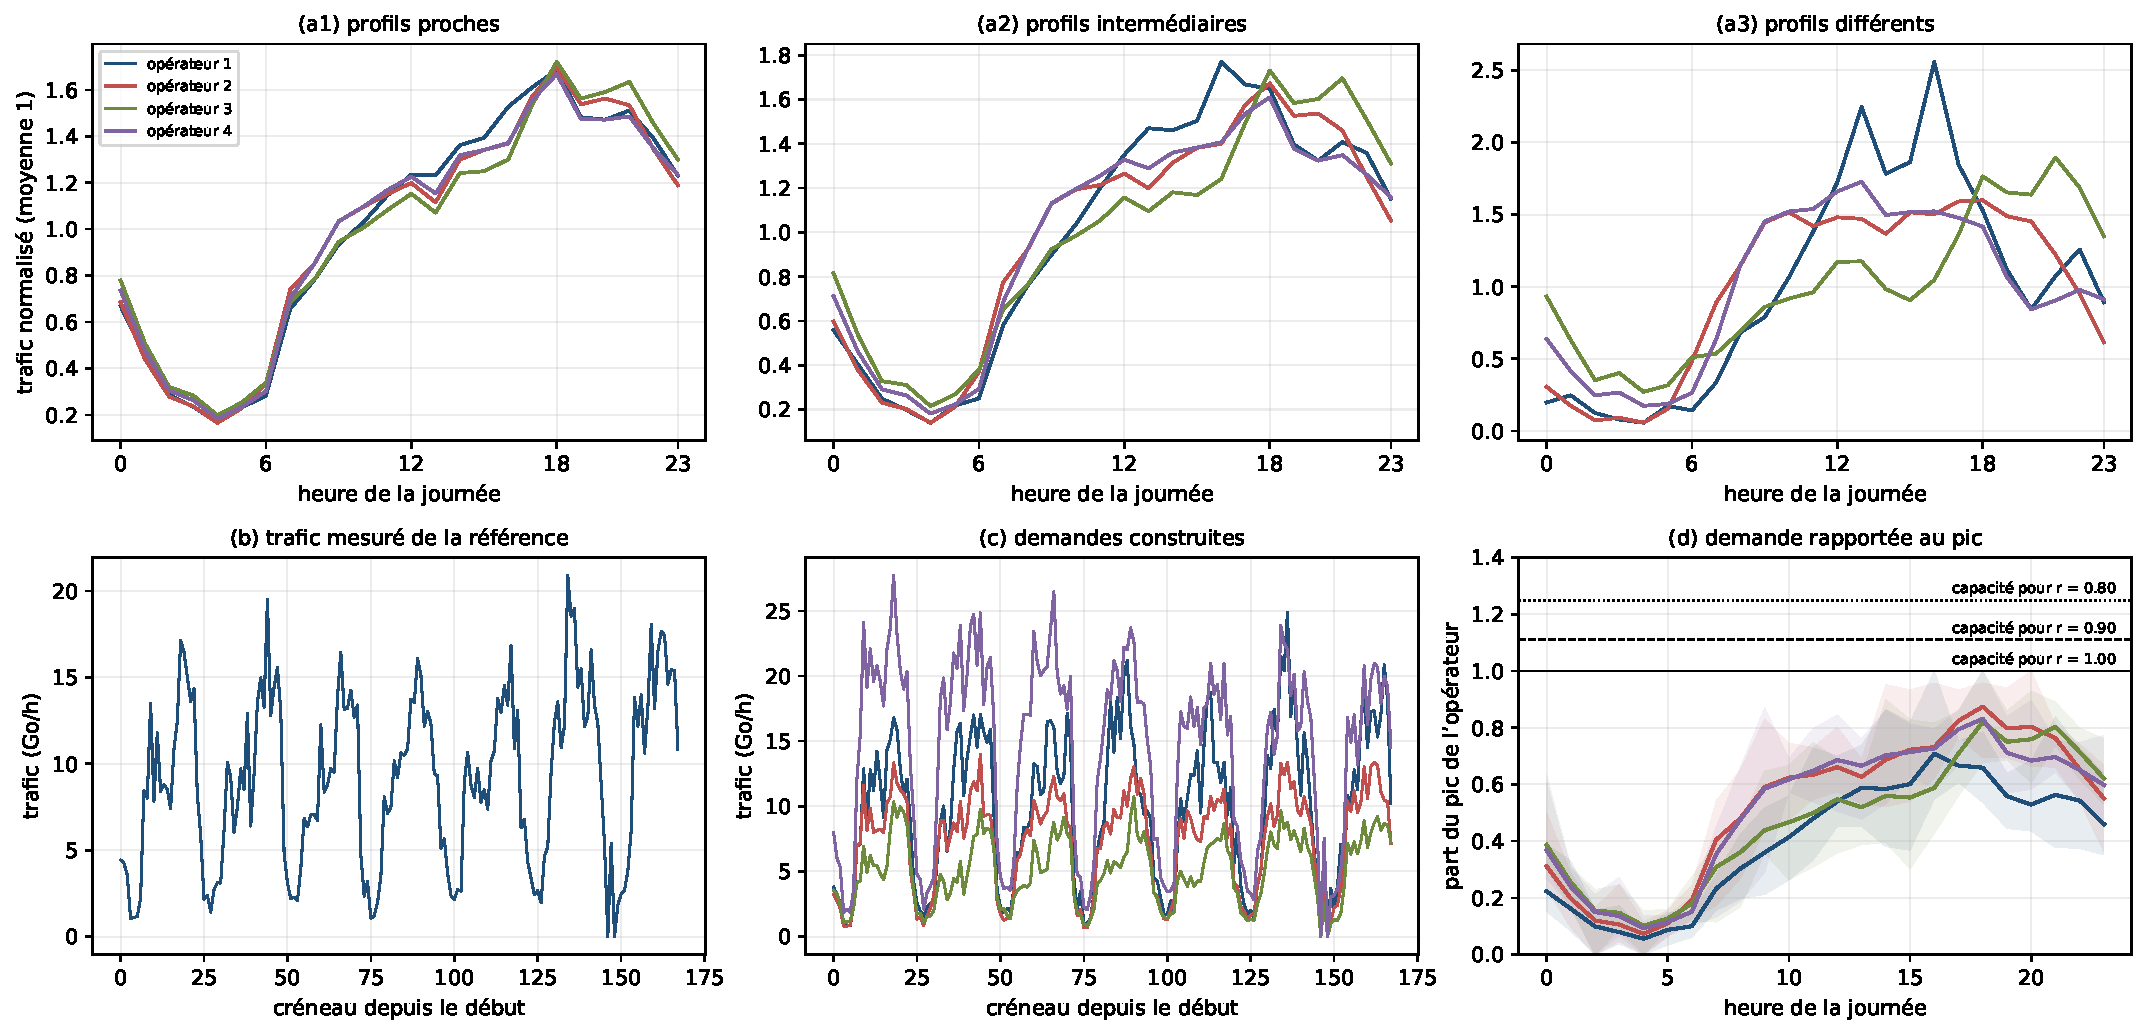
\includegraphics[width=0.98\textwidth]{../figures/protocol/plan_walkthrough.pdf}
    \caption{Construction d'un site virtuel. (a)--(c)~Profils proches,
    intermédiaires et différents, moyennés par heure de la journée ; les
    antennes sources et les volumes ne changent pas entre les trois panneaux.
    (d)~Série réelle de l'antenne de référence sur 168 heures.
    (e)~Les quatre demandes de la configuration intermédiaire construites
    par~\eqref{eq:demande_synthetique}.
    (f)~Demande rapportée au pic de chaque opérateur, plage des sept jours en
    zone colorée, et capacités correspondant aux trois valeurs de \(r\).}
    \label{fig:plan_deroule}
\end{figure}

\begin{table}[!htbp]
\centering
\small
\setlength{\tabcolsep}{3pt}
\begin{tabular}{lrrrr}
\hline
Opérateur & 1 & 2 & 3 & 4 \\
\hline
Antenne donneuse & \texttt{00000493U5} & \texttt{00000244W3} & \texttt{00024518W3} & \texttt{00000204U1} \\
Corrélation avec \(\phi_a\) & \(0{,}908\) & \(0{,}954\) & \(0{,}966\) & \(0{,}894\) \\
Facteur \(\alpha_i\) & \(1{,}087\) & \(0{,}797\) & \(0{,}555\) & \(1{,}562\) \\
Antenne d'énergie & \texttt{00000058W3} & \texttt{00000240U8} & \texttt{00083218W3} & \texttt{00000042U6} \\
\(P_i^{\mathrm{fixe}}\) (W) & \(1\,660{,}9\) & \(1\,758{,}7\) & \(1\,352{,}5\) & \(1\,563{,}7\) \\
Pente (W/Go) & \(41{,}85\) & \(28{,}86\) & \(26{,}62\) & \(24{,}51\) \\
Demande moyenne (Go/h) & \(9{,}96\) & \(7{,}30\) & \(5{,}08\) & \(14{,}31\) \\
Pic \(\max_t d_i(t)\) (Go/h) & \(24{,}90\) & \(13{,}97\) & \(10{,}73\) & \(27{,}70\) \\
\(q_i\) à \(r=0{,}90\) (Go/h) & \(27{,}66\) & \(15{,}52\) & \(11{,}92\) & \(30{,}78\) \\
\hline
\end{tabular}
\caption{Exemple de paramètres d'un site virtuel construit à partir de la
référence
\texttt{00083151W1}, d'échelle \(\mu_a=9{,}16\ \mathrm{Go/h}\). La somme des
demandes moyennes vaut \(36{,}65\ \mathrm{Go/h}\), soit exactement
\(4\mu_a\). Les chaînes alphanumériques sont les identifiants anonymisés des
antennes sources, et non des valeurs numériques.}
\label{tab:plan_deroule}
\end{table}
\FloatBarrier

\paragraph{Variantes contrôlées.}
Cinq réglages font varier les différences entre les opérateurs d'un même
plan : les volumes \(\alpha_i\), les profils temporels, les équipements, le
taux \(r\) et le nombre \(n\). La configuration de référence --- volumes et
profils intermédiaires, équipements issus du même quartile de puissance fixe,
\(r=0{,}90\), \(n=4\) --- est celle du Tableau~\ref{tab:plan_deroule}. On
modifie ensuite un réglage à la fois, en conservant le même plan. Les deux cas
où les trois premières dimensions sont toutes proches ou toutes très
différentes donnent seulement deux contrôles d'interaction.

La dispersion décrit ici les différences entre opérateurs à l'intérieur
d'une instance. Elle n'est pas synonyme de sensibilité : la sensibilité,
étudiée en Section~\ref{subsec:sensibilite_mecanismes}, mesure la variation
du résultat lorsqu'on change un réglage.

\paragraph{Capacités.}
La capacité n'est pas mesurée. On la fixe par un scénario, sous la
contrainte \(d_i^h\leqslant q_i\) de la
Section~\ref{subsec:fenetre_decision} : le pic de la demande construite
occupe une fraction \(r\) de la capacité,
\begin{equation}
    \max_{t\in\mathcal T}d_i(t)=r\,q_i,
    \qquad
    r\in\{0{,}80,\,0{,}90,\,1\}.
    \label{eq:capacite_scenario}
\end{equation}
Ainsi \(r=1\) pose \(q_i\) exactement au pic, et \(r<1\) laisse de la
marge. Changer \(r\) ne reconstruit pas les courbes de trafic : les trois
valeurs partagent les mêmes demandes, et seule la sélection des gardiens
--- quels équipements restent allumés --- peut changer. Par construction,
\(d_i(t)\leqslant r\,q_i\leqslant q_i\), donc aucune heure n'est
individuellement infaisable. Selon les réglages, le nombre minimal de
gardiens observé va de un à quatre ; la
Section~\ref{subsec:seuils_capacite_mecanisme} étudie directement ces quatre
cas.

\paragraph{Fenêtre, réplication et reproductibilité.}
La fenêtre centrale est
\[
    H=\{0\,\mathrm{h},1\,\mathrm{h},\ldots,6\,\mathrm{h}\},
\]
soit \([0\,\mathrm{h},7\,\mathrm{h})\), ses bornes étant un paramètre de
l'analyse de sensibilité. Conformément à~\eqref{eq:cout_horaire_principal},
les gardiens et l'allocation sont recalculés à chaque heure ; l'engagement
persistant de la Section~\ref{subsec:extension_persistante} est traité comme
une contrainte secondaire. Les \(168\) heures sont optimisées séparément, puis
résumées par heure de la journée. Les sept jours sont toujours traités
ensemble, conformément à la vérification donnée au début de cette
sous-section.

La liste gelée contient 400 plans, soit 400 sites virtuels par scénario ; il
ne s'agit pas de 400 sites multi-opérateurs observés. Les antennes de
référence sont tirées sans remise, à raison de 100 par quartile de trafic
moyen. Une graine unique fixe
l'ordre de tous les tirages. À
l'intérieur d'un plan, les sources de trafic et d'énergie sont disjointes ;
une antenne peut réapparaître dans plusieurs plans, jamais deux fois dans le
même. La stabilité des principaux résultats numériques est contrôlée en
comparant les deux moitiés de l'échantillon ; le plan reste toujours l'unité
d'observation.

\paragraph{Diagnostics et contrôles.}
Avant toute interprétation, l'espace d'instances simulé est comparé aux
données d'origine : profils journaliers, autocorrélation de décalage un,
corrélation entre opérateurs d'un même site, distributions des volumes, des
maxima, de \(F_i\) et de \(\gamma_i\), et fréquence des différentes valeurs de
\(k_h\). Ces diagnostics, ainsi que les contrôles croisés de l'implémentation,
sont reportés en Annexe~\ref{app:diagnostics_protocole}. Ces derniers
recalculent chaque optimum par deux méthodes indépendantes : la répartition
gloutonne de la Proposition~\ref{pro:opt} contre le programme
linéaire~\eqref{eq:lp_allocation_fixe}, l'énumération horaire contre le
programme mixte~\eqref{eq:milp_horaire}, la variante persistante
contre~\eqref{eq:milp_gardiens}, le test du cœur contre
Bondareva--Shapley~\eqref{eq:lp_bondareva_shapley}, et l'appartenance du
nucléole au moindre cœur~\eqref{eq:lp_moindre_coeur}. Les contre-exemples
analytiques des Propositions~\ref{prop:contre_exemple_coeur_vide}
et~\ref{prop:shapley_hors_coeur_semi_homogene} sont en outre reproduits
numériquement. Leur rôle est de vérifier que les résultats ne proviennent ni
d'une erreur de construction des instances ni d'une erreur d'implémentation.

\paragraph{Portée.}
Ces instances ne permettent pas d'estimer la distribution réelle des gains
d'un accord entre opérateurs colocalisés, et les capacités y sont
simulées. Elles autorisent en revanche une lecture comparative : à
plan fixé, mesurer comment l'efficacité et la stabilité réagissent lorsqu'on
déplace un seul facteur, tout en restant ancré sur des profils de trafic et
des équipements réellement mesurés.

\subsection{Modèle de puissance}
\label{subsec:adequation_modele_affine}

Le modèle suppose \(P_i(d)=P_i^{\mathrm{fixe}}+s_i d\) pour un équipement
actif. On l'ajuste par moindres carrés, antenne par antenne, sur les
heures à puissance strictement positive des sept jours. Une antenne est
écartée si le trafic ne varie pas, s'il y a trop peu d'heures actives, ou
si \(P^{\mathrm{fixe}}\) ou \(s\) n'est pas strictement positif. Il reste
\(3\,623\) antennes sur \(3\,825\).

L'erreur d'ajustement, rapportée à la puissance moyenne, vaut \(8{,}5\,\%\)
en médiane et reste sous \(15\,\%\) pour \(90\,\%\) des antennes. La part
fixe \(P^{\mathrm{fixe}}/(P^{\mathrm{fixe}}+s\,\bar d)\) vaut \(72\,\%\)
en médiane et dépasse la moitié pour \(93\,\%\) des antennes : éteindre un
équipement économise plus que le report de trafic n'en coûte.

La Figure~\ref{fig:ajustement_puissance} montre trois antennes distinctes,
aux quantiles \(25\,\%\), \(50\,\%\) et \(90\,\%\) de cette erreur :
(a)~bon, (b)~médian, (c)~médiocre. Rouge : \(0\,\mathrm{h}\)--\(6\,\mathrm{h}\) ;
bleu : reste de la journée.

\begin{figure}[htbp]
    \centering
    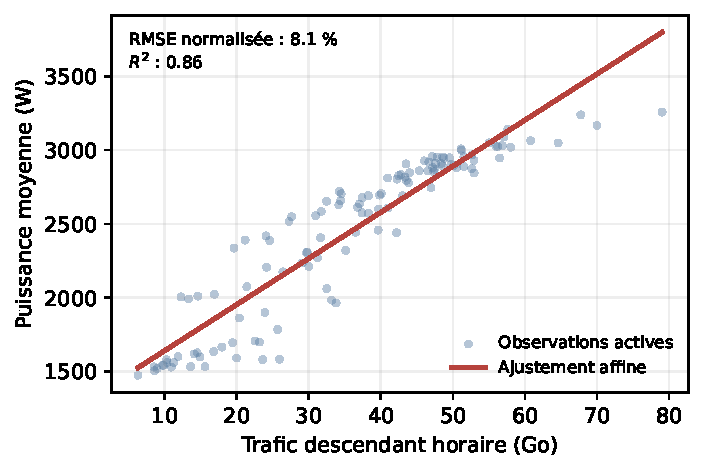
\includegraphics[width=0.95\textwidth]{../figures/power_calibration/representative_power_fit.pdf}
    \caption{Trois antennes distinctes, une par panneau. Droite : ajustement
    affine. Pointillé : \(P^{\mathrm{fixe}}\).}
    \label{fig:ajustement_puissance}
\end{figure}

L'ordonnée à l'origine \(P^{\mathrm{fixe}}\) est la puissance prédite lorsque
le trafic est nul. Elle ne repose pas sur un prolongement lointain de la
droite hors des observations : pour l'antenne médiane, le plus faible trafic
observé ne représente que \(1{,}7\,\%\) de son pic, et \(0{,}8\,\%\) des
heures où la puissance est positive ont exactement un trafic nul. Les données
contiennent donc des points au voisinage immédiat de l'origine.

\paragraph{Deux régimes lorsque l'équipement est actif.}
Le panneau (c), à droite, présente deux groupes de points. Pour un même
niveau de trafic, la puissance mesurée entre 0 h et 6 h est plus faible que
celle mesurée entre 7 h et 23 h ; le rapport entre la seconde et la première
vaut \(1{,}43\) en médiane. Aucune des deux n'est
\(P^{\mathrm{fixe}}\) : ce sont des puissances mesurées pendant que
l'équipement transporte du trafic, tandis que \(P^{\mathrm{fixe}}\) est
l'ordonnée à l'origine de la droite pointillée. Environ \(80\,\%\) des
antennes présentent ce changement de niveau selon l'heure. Le modèle des
Sections 3 à 5 ne distingue qu'un état actif et un état sans trafic ; nous
conservons donc une seule droite par antenne, ajustée sur les 168 heures.

\paragraph{Passage aux coûts.}
On pose \(F_i=\pi P_i^{\mathrm{fixe}}\) et \(\gamma_i=\pi s_i\), avec
\(\pi\) le prix de l'électricité, identique pour tous. Un facteur commun
ne change ni les gardiens ni les économies relatives : on rapporte les
résultats en énergie.

\subsection{Efficacité opérationnelle}
\label{subsec:efficacite_operationnelle}

Cette sous-section étend le calcul du plan déroulé aux 400 plans de
la liste gelée. Pour chacune des trois valeurs de \(r\), cela représente
\(400\) plans observés pendant sept jours, donc \(2\,800\) simulations
journalières. Pour chaque plan et chaque jour, les vingt-quatre coûts
\(C_h^*(N)\) sont obtenus par énumération des quinze ensembles de gardiens et
répartition gloutonne de la Proposition~\ref{pro:opt}.

Nous réutilisons directement le jeu défini en~\eqref{eq:jeu_principal} :
\(v_h(N)\), converti en kWh, est l'énergie économisée par rapport au
fonctionnement autonome, et
\(v_h(N)/\sum_i C_h^*(\{i\})\) est la part économisée. Il n'y a donc pas de
nouveau point de comparaison : le dénominateur reste le coût autonome défini
en Section~\ref{sec:jeu_cooperatif}. Chaque résultat est d'abord
moyenné sur les sept jours d'un plan, puis résumé sur les 400 plans. Dans
les tableaux, les crochets contiennent directement la moitié centrale des
plans, du premier au troisième quartile ; aucun rééchantillonnage ni intervalle
de confiance n'est utilisé.

\paragraph{Profil horaire et choix de \(H\).}
La Figure~\ref{fig:efficacite_operationnelle} suit simultanément la part et
la quantité économisée et le nombre de gardiens effectivement retenus par
l'optimum, \(|G_h^*(N)|\). Les volumes et les profils sont au niveau modéré de
la grille ; les quatre équipements sont tirés dans le même quartile de
\(P^{\mathrm{fixe}}\), avec \(n=4\) et \(r=0{,}90\). Les sept jours sont
traités ensemble selon le protocole de la
Section~\ref{subsec:protocole_experimental}. Le nombre minimal d'équipements
imposé par les seules capacités, \(k_h\), et les conditions suffisantes de
stabilité sont étudiés séparément en
Section~\ref{subsec:seuils_capacite_mecanisme}.

La part économisée médiane vaut \(67{,}6\,\%\) à minuit,
\(76{,}0\,\%\) à 5 h et \(43{,}3\,\%\) à 18 h. L'énergie économisée varie
moins, de \(2{,}22\) à \(3{,}00\,\mathrm{kWh}\) par heure : en journée, le
trafic accroît à la fois le coût du fonctionnement autonome et le nombre de
gardiens retenus par l'optimum.
Le nombre moyen proche de deux vers 18 h signifie seulement que, dans ces
sites virtuels, les capacités simulées de deux équipements suffisent le plus
souvent à servir la demande totale. Il ne s'agit pas d'une mesure du nombre
d'équipements nécessaires sur un site réel.

\begin{figure}[htbp]
    \centering
    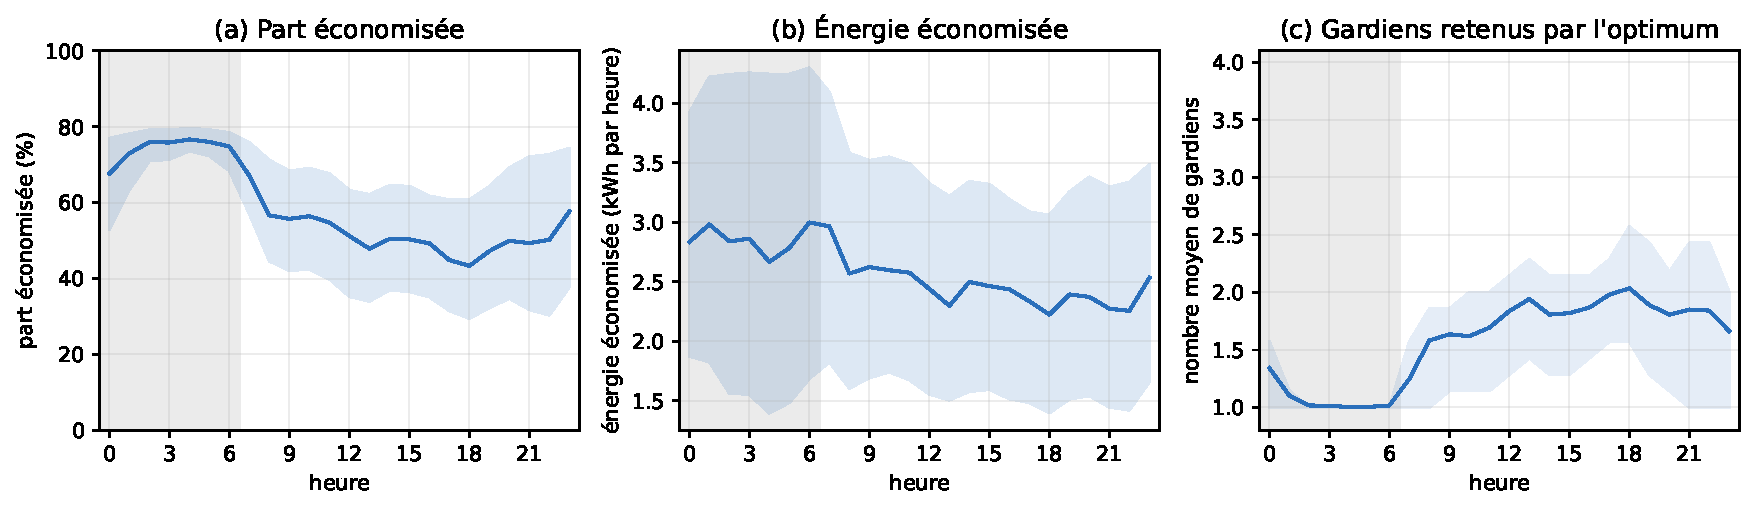
\includegraphics[width=\textwidth]{../figures/operational_efficiency/hourly_profiles.pdf}
    \caption{Profil horaire sur 400 plans, \(r=0{,}90\), les sept jours
    regroupés. (a)--(b)~Part et quantité économisée par rapport au
    fonctionnement autonome. (c)~Nombre de gardiens de l'ensemble choisi par
    l'optimum. Les courbes donnent la médiane des plans et les zones colorées
    leur moitié centrale ; la zone grise est la fenêtre nocturne étudiée.}
    \label{fig:efficacite_operationnelle}
\end{figure}

La fenêtre \(H=\{0,\ldots,6\}\), représentée en gris, a été fixée avant ces
résultats et non choisie en fonction du niveau d'économie observé.

\paragraph{Fenêtre et capacité.}
Le Tableau~\ref{tab:plan_quatre_r} compare les mêmes demandes pour les trois
valeurs de capacité fixées par~\eqref{eq:capacite_scenario}. Accroître \(r\)
de \(0{,}80\) à \(1\) réduit la part économisée de \(1{,}1\) point ; l'énergie
économisée varie de moins de \(0{,}8\,\mathrm{kWh}\) par nuit.

Dans les tableaux de cette sous-section, la notation
\(m\,[q_{25};q_{75}]\) donne la médiane \(m\), puis les premier et troisième
quartiles. Par exemple, \(73{,}7\,[66{,}5;78{,}3]\) signifie que la médiane
des 400 plans vaut \(73{,}7\,\%\) et que leur moitié centrale se trouve
entre \(66{,}5\,\%\) et \(78{,}3\,\%\).

\begin{table}[htbp]
\centering
\small
\setlength{\tabcolsep}{4pt}
\begin{tabular}{ccc}
\hline
\(r\) & Part économisée (\%) & Énergie économisée (kWh/nuit) \\
\hline
\(0{,}80\) & \(74{,}4\ [67{,}1;78{,}4]\) & \(20{,}5\ [11{,}9;29{,}9]\) \\
\(0{,}90\) & \(73{,}7\ [66{,}5;78{,}3]\) & \(20{,}0\ [11{,}9;29{,}6]\) \\
\(1\)      & \(73{,}3\ [65{,}6;78{,}0]\) & \(19{,}7\ [11{,}8;29{,}3]\) \\
\hline
\end{tabular}
\caption{Résultats médians sur les sept nuits. Les crochets contiennent la
moitié centrale des 400 plans. Les demandes sont identiques entre les
lignes.}
\label{tab:plan_quatre_r}
\end{table}

À \(r=0{,}90\), le fonctionnement autonome consomme en médiane
\(30{,}2\,\mathrm{kWh}\) par nuit, contre \(7{,}9\,\mathrm{kWh}\) à
l'optimum. Cet écart est grand parce que le modèle autorise l'extinction
complète : l'optimum ne garde qu'un équipement dans \(93{,}4\,\%\) des heures
nocturnes et évite alors l'essentiel des trois autres coûts fixes. Le terme
fixe représente en médiane \(88{,}6\,\%\) de l'énergie du fonctionnement
autonome sur \(H\). Les quatre puissances fixes sont comparables : la plus
petite représente \(21{,}4\,\%\) de leur somme, contre \(25\,\%\) si elles
étaient identiques. La valeur de \(73{,}7\,\%\) est donc cohérente avec trois
extinctions sur quatre sous les hypothèses du modèle ; elle ne constitue pas
une économie mesurée sur un site réel.

\paragraph{Nombre d'opérateurs.}
Sur les mêmes 400 plans à \(r=0{,}90\), la part économisée passe de
\(66{,}5\,\%\ [59{,}7;70{,}5]\) pour les trois premiers opérateurs à
\(73{,}7\,\%\ [66{,}5;78{,}3]\) pour quatre. La différence appariée médiane
vaut \(6{,}8\ [4{,}6;8{,}1]\) points. Ces valeurs sont proches des
repères homogènes \((n-1)/n\), soit \(66{,}7\,\%\) et \(75\,\%\), car les
puissances fixes sont comparables.

\paragraph{Politiques de référence.}
Trois comparaisons complètent l'optimum horaire. La première allume, à chaque
heure, les équipements par capacité décroissante jusqu'à couvrir la demande,
puis répartit le trafic au moindre coût variable entre eux. La deuxième garde
les équipements de l'optimum, mais répartit le trafic au prorata de leurs
capacités. La troisième impose le même ensemble de gardiens pendant les sept
heures de la nuit, comme dans l'extension persistante de la
Section~\ref{subsec:extension_persistante}.

Pour chaque politique, la Figure~\ref{fig:plan_capacite} contient 400
valeurs : une par plan, après moyenne de ses sept nuits. Le
Tableau~\ref{tab:politiques_operationnelles} résume les comparaisons
appariées plan par plan. Choisir en priorité les équipements de plus grande
capacité ignore leurs coûts et réduit la part économisée de \(3{,}4\) points
en médiane. Imposer le même ensemble de gardiens pendant toute la nuit la
réduit de \(3{,}2\) points.

Les 400 plans utilisent le même réglage, mais pas les mêmes antennes de
référence, donneuses et énergétiques. Pour l'optimum, la moitié centrale des
économies absolues va ainsi de \(11{,}9\) à \(29{,}6\,\mathrm{kWh}\) par nuit.
La part économisée varie moins entre plans, car elle rapporte cette énergie à
la consommation autonome du même plan. Pour la règle par capacité, quatre
plans sur 400 ont même une économie moyenne négative : ignorer les coûts fixes
et variables peut sélectionner des équipements dont la consommation dépasse
la référence autonome. Ces quatre extrêmes sont conservés dans les calculs,
mais pas dans l'échelle des moustaches de la figure.

La politique proportionnelle conserve, à chaque heure, exactement les gardiens trouvés par l'optimum, puis
répartit seulement le trafic entre eux au prorata de leur capacité. Or
\(|G_h^*(N)|=1\) dans \(93{,}4\,\%\) des heures nocturnes : la répartition est
alors imposée et les deux politiques coïncident. Sur les autres heures, la
perte médiane de la répartition proportionnelle vaut \(1{,}14\) point. Son bon
résultat global vient donc surtout du choix préalable des gardiens optimaux,
et non d'une optimalité générale de la règle proportionnelle.

\begin{figure}[htbp]
    \centering
    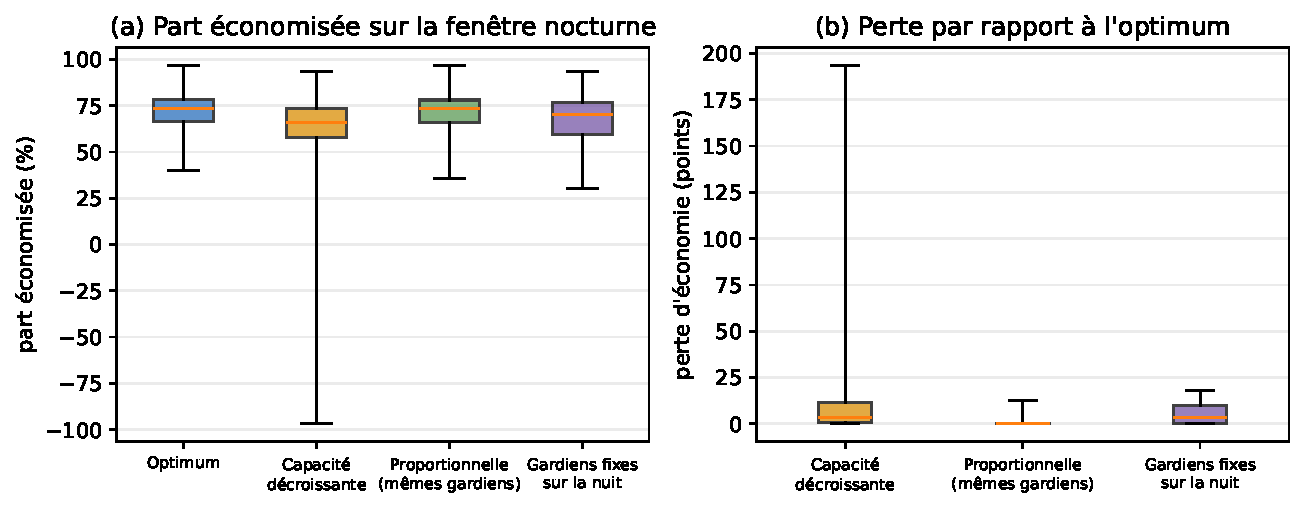
\includegraphics[width=\textwidth]{../figures/operational_efficiency/operational_efficiency.pdf}
    \caption{Résultats des quatre politiques sur 400 plans. Chaque boîte
    résume 400 moyennes, une par plan sur ses sept nuits : le trait orange
    est la médiane, la boîte contient la moitié centrale des plans et les
    moustaches vont des 5\textsuperscript{e} aux 95\textsuperscript{e} centiles.
    (a)~Part économisée par rapport
    au fonctionnement autonome. (b)~Perte appariée par rapport à l'optimum
    horaire.}
    \label{fig:plan_capacite}
\end{figure}

\begin{table}[htbp]
\centering
\setlength{\tabcolsep}{3pt}
\begin{tabular}{lcc}
\hline
Politique & Part économisée (\%) & Perte (points) \\
\hline
Optimum horaire & \(73{,}7\ [66{,}5;78{,}3]\) & --- \\
Capacité décroissante & \(66{,}2\ [57{,}6;73{,}6]\) & \(3{,}4\ [0{,}6;11{,}3]\) \\
Répartition proportionnelle & \(73{,}6\ [65{,}7;78{,}1]\) & \(0{,}002\ [0;0{,}127]\) \\
Gardiens fixes sur la nuit & \(70{,}1\ [59{,}2;76{,}8]\) & \(3{,}2\ [0{,}01;9{,}8]\) \\
\hline
\end{tabular}
\caption{Médianes des 400 plans à \(r=0{,}90\). Les crochets contiennent la
moitié centrale des plans. La perte est calculée plan par plan avant d'en
prendre la médiane ; ce n'est pas la différence entre les deux médianes de la
colonne précédente.}
\label{tab:politiques_operationnelles}
\end{table}

La perte proportionnelle médiane de \(0{,}002\) point est positive mais
presque nulle. Elle ne se déduit pas de \(73{,}7-73{,}6\), car les deux
médianes de la première colonne sont calculées séparément, tandis que la
perte est calculée plan par plan avant d'en prendre la médiane.

L'optimum change d'ensemble \(1{,}14\) fois par nuit en médiane et reste
constant dans \(40{,}6\,\%\) des nuits simulées. La moitié centrale des pertes
dues à la contrainte persistante va de \(0{,}01\) à \(9{,}8\) points : la
reconfiguration horaire importe donc pour une partie des plans.

\paragraph{Année et temps de calcul.}
La moyenne directe des sept nuits observées donne une énergie économisée
médiane de \(20{,}0\,\mathrm{kWh}\) par site et par nuit ; la moitié centrale
des plans va de \(11{,}9\) à \(29{,}6\,\mathrm{kWh}\).
Répétée 365 fois, elle donne \(7{,}3\,\mathrm{MWh}\) par site et par an,
avec une moitié centrale de \(4{,}3\) à \(10{,}8\,\mathrm{MWh}\). La
saisonnalité n'étant pas observée,
il s'agit seulement d'un ordre de grandeur.
Sur la machine de calcul, un site-jour complet --- profil 24 h, trois
politiques et persistance sur \(H\) --- prend environ \(11\,\mathrm{ms}\) pour
\(n=3\) et \(14\,\mathrm{ms}\) pour \(n=4\) ; les \(8\,400\) simulations
journalières sont résolues en environ \(171\,\mathrm{s}\), hors chargement et tracé. Les
résultats intermédiaires sont enregistrés et réutilisés tant que les données,
le protocole et le code de calcul n'ont pas changé.

\subsection{Stabilité et répartition des économies}
\label{subsec:stabilite_grande_coalition}

Nous conservons les 400 plans et les sept heures de \(H\), mais examinons
ici le jeu horaire \(v_h\). Une observation est donc définie par un plan, un
jour, une heure et une valeur de \(r\). Les 400 plans, les sept jours, les
sept heures et les trois valeurs \(r\in\{0{,}80,0{,}90,1\}\) fournissent
\(400\times7\times7\times3=58\,800\) jeux appariés. Cette granularité étudie
une rupture heure par heure. Un cœur vide pour un jeu \(v_h\) n'implique pas
un cœur vide pour le jeu \(v_H\) de la nuit entière : l'agrégation permet aux
gains de différentes heures de compenser leurs contraintes coalitionnelles.
Les deux diagnostics répondent donc à des questions différentes.
Une solution pratique consiste à régler les transferts sur une période plus
longue. Lorsque les 49 heures nocturnes des sept jours sont réunies dans un
seul jeu par plan, aucun des \(400\times3=1\,200\) cœurs n'est vide. À
\(r=0{,}90\), Shapley appartient au cœur pour 378 plans et un autre partage
stable existe pour les 22 autres. L'instabilité horaire ne persiste donc pas
nécessairement lorsque les comptes sont faits en fin de semaine.

\paragraph{Cascade.}
Le test d'appartenance de Shapley au cœur conclut directement pour \(51\,046\)
jeux, soit \(86{,}8\,\%\). Les
\(7\,754\) autres passent au test de non-vacuité du cœur : \(4\,419\) ont un
cœur non vide et \(3\,335\) un cœur vide. Le nucléole n'est calculé que dans
les \(4\,419\) premiers cas, afin d'obtenir le partage stable retenu ; il ne
l'est jamais si Shapley convient déjà. Lorsque le cœur est vide, l'analyse de
la rupture est séparée et le nucléole n'est pas utilisé comme prédiction de
coalition. Sur l'ensemble des 400 plans, le test de Shapley prend \(7{,}3\)
secondes pour les \(58\,800\) jeux et le test du cœur \(17{,}8\) secondes pour
les \(7\,754\) jeux qui l'atteignent, contre \(545\) secondes pour les
\(4\,419\) nucléoles. Ce
dernier étage domine le calcul. Les diagnostics et les partages sont
enregistrés et réutilisés tant que les entrées et le code ne changent pas.

\paragraph{Trois catégories.}
Le Tableau~\ref{tab:stabilite_grande_coalition} donne la répartition des trois
cas. La fréquence de cœur vide passe de \(4{,}6\,\%\) à \(6{,}7\,\%\) lorsque
\(r\) passe de \(0{,}80\) à \(1\), c'est-à-dire lorsque les capacités
\(q_i=\max_t d_i(t)/r\) diminuent. Entre les deux moitiés de 200 plans, l'écart maximal
entre les fréquences des trois catégories n'est plus que de \(1{,}4\) point.

\begin{table}[htbp]
\centering
\setlength{\tabcolsep}{4pt}
\begin{tabular}{ccccc}
\hline
\(r\) & Jeux & \shortstack{Shapley\\stable} &
\shortstack{Autre partage\\stable} &
\shortstack{Grande coalition\\instable} \\
\hline
\(0{,}80\) & \(19\,600\) & \(17\,313\ (88{,}3\,\%)\) & \(1\,378\ (7{,}0\,\%)\) & \(909\ (4{,}6\,\%)\) \\
\(0{,}90\) & \(19\,600\) & \(17\,014\ (86{,}8\,\%)\) & \(1\,477\ (7{,}5\,\%)\) & \(1\,109\ (5{,}7\,\%)\) \\
\(1\) & \(19\,600\) & \(16\,719\ (85{,}3\,\%)\) & \(1\,564\ (8{,}0\,\%)\) & \(1\,317\ (6{,}7\,\%)\) \\
\textbf{Total} & \(58\,800\) & \(51\,046\ (86{,}8\,\%)\) & \(4\,419\ (7{,}5\,\%)\) & \(3\,335\ (5{,}7\,\%)\) \\
\hline
\end{tabular}
\caption{Répartition des jeux horaires de la fenêtre \(H\), sur 400 plans
et avec \(n=4\). « Autre partage stable » signifie que le cœur est non vide
mais que Shapley n'y appartient pas ; le partage retenu est alors le
nucléole.}
\label{tab:stabilite_grande_coalition}
\end{table}

\paragraph{Amplitude de l'instabilité.}
Seuls \(390\) des \(58\,800\) jeux sont convexes, alors que \(86{,}8\,\%\)
admettent Shapley dans le cœur : la convexité est bien une condition
suffisante, non nécessaire. Lorsque le cœur est vide, il faudrait autoriser
chaque coalition à recevoir jusqu'à \(5{,}2\,\%\) de moins que sa contrainte
de stabilité, en médiane, pour rendre un partage possible ; la moitié centrale
de ce manque minimal va de \(2{,}6\) à \(8{,}5\,\%\) de l'économie totale.
Lorsque le cœur est non vide mais exclut Shapley, l'objection
maximale à ce partage vaut \(2{,}77\,\%\) de l'économie en médiane. La
coalition qui objecte compte trois opérateurs dans \(76{,}9\,\%\) des cas et
deux dans les autres. Un test simplifié additionne les exigences des quatre
sous-groupes de trois opérateurs, chacun obtenu en retirant un opérateur. Si
leur somme dépasse ce que la grande coalition peut distribuer, le cœur est
nécessairement vide. Ce test détecte \(65{,}7\,\%\) des cœurs vides, sans faux
positif.

\paragraph{Gains distribués et benchmark de rupture.}
À \(r=0{,}90\), nous additionnons, pour chaque opérateur, les gains qui lui
sont attribués aux sept heures de la nuit. Sur
les \(1\,600\) couples plan--opérateur, le gain moyen est
\(5{,}06\,\mathrm{kWh}\) par nuit, soit \(0{,}76\) euro par opérateur au prix
de \(0{,}15\) euro/kWh, ou \(3{,}04\) euros pour les quatre opérateurs du site.
La médiane est \(5{,}20\,\mathrm{kWh}\) et la moitié
centrale va de \(2{,}90\) à \(7{,}25\,\mathrm{kWh}\). Les numéros
d'opérateur n'étant pas comparables d'un plan à l'autre, nous ne donnons pas
quatre moyennes par identité ; au sein d'un plan, les gains moyens des rangs
le plus faible et le plus élevé valent respectivement \(4{,}49\) et
\(5{,}89\,\mathrm{kWh}\) par nuit.

Lorsque le cœur est vide, le jeu ne prédit pas à lui seul la coalition qui se
formera. Comme benchmark, nous énumérons toutes les partitions propres des
quatre opérateurs, vérifions la stabilité du partage au sein de chaque groupe,
puis retenons la partition stable qui conserve le plus d'économies. Ce
scénario de meilleure partition stable quantifie une perte potentielle ; ce
n'est pas un modèle de formation des coalitions. La perte est mesurée par
rapport au partage de Shapley, hypothétique, de la grande coalition. À
\(r=0{,}90\), les \(1\,109\) cœurs vides sur \(19\,600\) jeux perdent en moyenne
\(0{,}159\,\mathrm{kWh}\) pendant l'heure concernée, avec une médiane de
\(0{,}075\,\mathrm{kWh}\). Cette perte représente en moyenne \(5{,}6\,\%\) de
l'économie de la grande coalition pendant les heures concernées, avec une
médiane de \(4{,}0\,\%\). Rapportée aux \(2\,800\) nuits, ruptures ou non, la
perte collective moyenne est \(0{,}063\,\mathrm{kWh}\) par site et par nuit.
La perte moyenne par opérateur est \(0{,}016\,\mathrm{kWh}\) par nuit ; sa
médiane est nulle et les 5\textsuperscript{e}--95\textsuperscript{e} centiles
vont de \(-0{,}119\) à \(0{,}212\,\mathrm{kWh}\). Une valeur négative signifie
que certains opérateurs bénéficient de la rupture, même si la perte totale est
toujours positive.

Le panneau (b) de la Figure~\ref{fig:stabilite_grande_coalition} ne compare
pas trois politiques énergétiques : dans les trois boîtes, l'économie est
celle de la grande coalition optimale. Les jeux sont seulement classés après
calcul selon leur diagnostic de stabilité ; une économie plus grande ne
garantit donc pas un partage stable.

\begin{figure}[htbp]
    \centering
    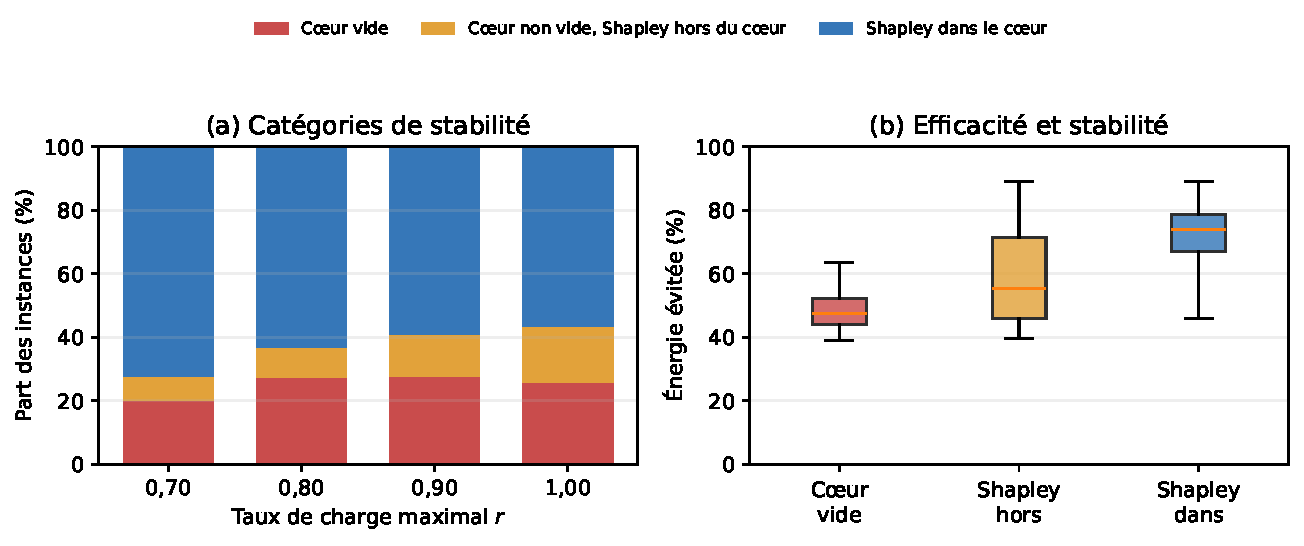
\includegraphics[width=\textwidth]{../figures/coalition_stability/coalition_stability.pdf}
    \caption{Stabilité des \(58\,800\) jeux horaires. (a)~Répartition des trois
    diagnostics selon le taux de charge maximal. (b)~Énergie économisée par
    la grande coalition pendant une heure, c'est-à-dire \(v_h(N)\), classée
    selon le diagnostic. Chaque boîte montre la médiane, la moitié centrale
    et les 5\textsuperscript{e}--95\textsuperscript{e} centiles. Le rouge
    indique un cœur vide, donc une grande coalition instable ; les boîtes ne
    représentent pas des politiques différentes.}
    \label{fig:stabilite_grande_coalition}
\end{figure}

\FloatBarrier

\subsection{Nombre minimal de gardiens et mécanisme}
\label{subsec:seuils_capacite_mecanisme}

La somme sur toute la nuit calculée dans la sous-section précédente peut
masquer les changements du nombre d'équipements nécessaires. Nous revenons
donc au jeu horaire \(v_h\). Pour chacun des 400 plans, nous combinons la
configuration de référence --- volumes et profils intermédiaires, équipements
de puissances fixes proches --- et une configuration où volumes, profils et
équipements sont tous proches. Chacune est évaluée avec les trois valeurs de
\(r\), les sept jours et les 24 heures. Un jeu horaire
est ici entièrement déterminé par un plan et l'une de ces combinaisons. Il y
en a donc
\(400\times2\times3\times7\times24=403\,200\) pour \(n=4\). Le même calcul est
effectué avec les trois premiers opérateurs de chaque plan, soit
\(403\,200\) jeux supplémentaires pour \(n=3\).

Pour interpréter ces jeux, on classe les capacités par ordre décroissant et
on note \(k_h\) le plus petit nombre des équipements les plus capacitaires
dont la capacité cumulée couvre le trafic total à l'heure \(h\). Ainsi,
\(k_h=3\) signifie précisément que les deux plus grandes capacités ne
suffisent pas, mais que les trois plus grandes suffisent. Ce classement
donne un minimum technique, pas le nombre de gardiens effectivement choisi.
L'ensemble \(G_h^*(N)\) peut contenir davantage d'équipements si cela réduit
le coût variable malgré un coût fixe supplémentaire. Ce classement décrit le
régime de charge observé ; il ne constitue pas, à lui seul, une preuve que le
changement de \(k_h\) cause l'instabilité.

\paragraph{Très faible trafic.}
La condition suffisante
\(d^h(N)\leqslant\min_i q_i\) du
Théorème~\ref{thm:capacite_coeur_non_vide} s'applique à
\(138\,200\) jeux à quatre opérateurs (\(34{,}3\,\%\)) et à \(173\,354\) jeux à
trois opérateurs (\(43{,}0\,\%\)). Aucun de ces \(311\,554\) jeux n'a un cœur
vide. Ces pourcentages portent sur les \(403\,200\) observations horaires de
chaque taille de coalition, et non sur 400 plans ou sur des nuits entières.
Dans la configuration de
référence, l'heure la plus favorable est 4 h : la condition est satisfaite
pour \(93{,}4\,\%\) des \(8\,400\) combinaisons plan--jour--\(r\) lorsque \(n=4\),
et pour \(98{,}2\,\%\) lorsque \(n=3\). Les heures 2--6 h sont les plus
favorables dans les deux cas. La condition locale de la
Remarque~\ref{prop:sousadd_stricte_locale}, plus faible, n'est pas comptée ici.

\begin{table}[htbp]
\centering
\begin{tabular}{ccrrr}
\hline
Opérateurs & Gardiens minimaux & Jeux horaires & Cœur vide &
Shapley dans le cœur \\
\hline
3 & 1 & 255\,104 & 2,1\,\% & 94,1\,\% \\
3 & 2 & 128\,992 & 36,0\,\% & 43,5\,\% \\
3 & 3 & 19\,104 & 0,0\,\% & 84,0\,\% \\
\hline
4 & 1 & 219\,194 & 5,5\,\% & 86,1\,\% \\
4 & 2 & 122\,802 & 38,9\,\% & 15,4\,\% \\
4 & 3 & 53\,505 & 59,0\,\% & 20,4\,\% \\
4 & 4 & 7\,699 & 0,0\,\% & 64,1\,\% \\
\hline
\end{tabular}
\caption{Diagnostic des 400 plans selon le nombre minimal de gardiens. Chaque
pourcentage est conditionnel à la ligne correspondante ; la colonne
\emph{Jeux horaires} en donne le dénominateur.}
\label{tab:seuils_capacite}
\end{table}

\paragraph{Nombre minimal de gardiens.}
Le tableau sert à localiser les cœurs vides selon le régime de charge. Par
exemple, \(38{,}9\,\%\) ne concerne que les \(122\,802\) jeux à quatre
opérateurs avec \(k_h=2\), et non l'ensemble des jeux. La fréquence atteint
\(59{,}0\,\%\) pour \(k_h=3\), soit \(31\,572\) cas sur \(53\,505\). Tous
régimes confondus, \(91\,352\) des \(403\,200\) jeux à quatre opérateurs ont
un cœur vide, soit \(22{,}7\,\%\). Ces fréquences sont élevées parce que cette
campagne inclut les 24 heures, trois capacités et deux configurations, et pas
seulement la fenêtre nocturne de référence de la
Section~\ref{subsec:stabilite_grande_coalition}.

Le mécanisme reste celui du contre-exemple théorique : chacun des quatre
sous-groupes de trois opérateurs peut exiger une économie importante, alors
qu'un opérateur appartient à trois de ces sous-groupes. La grande coalition
peut alors manquer d'économies pour satisfaire simultanément les quatre
contraintes. Le test simplifié fondé sur ces quatre sous-groupes
détecte \(76{,}7\,\%\) des cœurs vides pour \(n=4\). Lorsque Shapley est
contestée, la coalition qui présente l'objection maximale est une paire dans
\(37{,}0\,\%\) des cas et un triplet dans \(63{,}0\,\%\). Le cœur vide traduit
une impossibilité de partager les gains de manière stable, non une
infaisabilité technique du service.

Avec trois opérateurs, la condition de très faible trafic est effectivement
plus fréquente et Shapley est stable dans \(77{,}4\,\%\) des jeux, contre
\(55{,}4\,\%\) avec quatre ; le cœur est non vide dans \(87{,}1\,\%\) des
cas, contre \(77{,}3\,\%\). Le gain collectif moyen est en revanche plus
faible : \(1{,}75\,\mathrm{kWh}\) pendant une heure au lieu de
\(2{,}60\,\mathrm{kWh}\). Le cas \(n=3\) confirme donc, sur cet échantillon,
l'intuition d'une stabilité plus fréquente en contrepartie d'un gain total
plus petit. Le lien n'est toutefois pas monotone dans \(k_h\) et le tableau
n'établit pas d'effet causal du nombre minimal de gardiens.

\paragraph{Homogénéité des coûts.}
Nous remplaçons, dans chaque jeu à quatre opérateurs, tous les \(F_i\) par leur
moyenne et tous les \(\gamma_i\) par leur moyenne, puis réintroduisons 25, 50,
75 et 100\,\% des écarts aux moyennes. Le niveau 0\,\% donne donc quatre
opérateurs aux coûts identiques, et 100\,\% restitue les coûts initiaux. Sous
la condition de très faible
trafic, Shapley appartient au cœur dans 100\,\% des jeux à coûts identiques,
comme le garantit le
Corollaire~\ref{cor:shapley_coeur_tres_faible_trafic_homogene}. Cette fréquence
reste supérieure à 99\,\% à 25 et 50\,\% de dispersion, puis tombe à 98,2 et
96,4\,\%. Dès que les coûts diffèrent, le corollaire ne fournit plus de
garantie ; le contre-exemple théorique montre précisément qu'une exception
est alors possible. Sur
toutes les heures, sa fréquence passe de 73,5\,\% à coûts identiques à
60,6\,\% dès le premier quart de dispersion, puis atteint 55,4\,\% avec la
dispersion complète.

\begin{figure}[htbp]
    \centering
    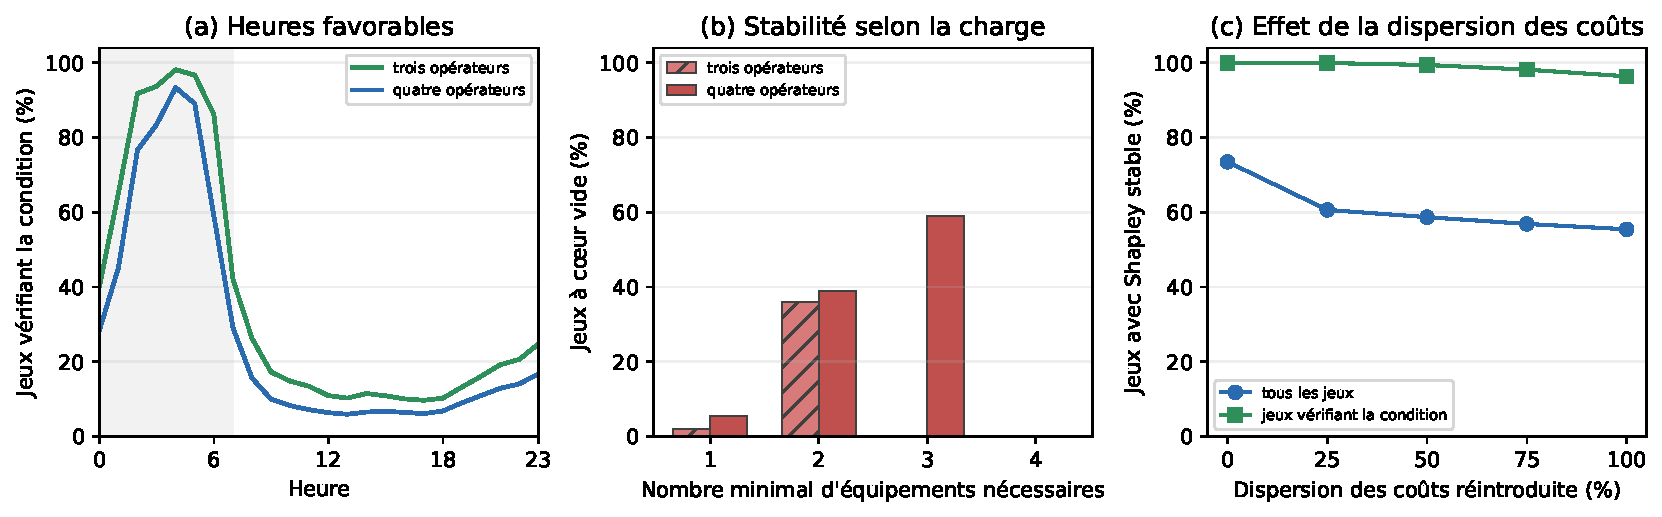
\includegraphics[width=\textwidth]{../figures/coalition_stability/threshold_mechanisms.pdf}
    \caption{Charge et stabilité sur les 400 plans. (a)~Part des \(8\,400\)
    combinaisons plan--jour--\(r\) qui satisfont la condition de très faible
    trafic dans la configuration de référence, selon l'heure et le nombre
    d'opérateurs ; la zone grise indique la fenêtre nocturne.
    (b)~Pour chaque nombre minimal d'équipements nécessaires, part des jeux
    de cette catégorie dont le cœur est vide ; les effectifs sont donnés dans le
    Tableau~\ref{tab:seuils_capacite}.
    (c)~Part des jeux où Shapley appartient au cœur quand les coûts passent
    d'identiques (0\,\%) aux coûts initiaux (100\,\%). La courbe verte porte seulement
    sur les \(138\,200\) jeux de très faible trafic ; seule sa valeur au point
    homogène est garantie par le corollaire.}
    \label{fig:seuils_mecanisme}
\end{figure}

\FloatBarrier

\subsection{Sensibilité}
\label{subsec:sensibilite_mecanismes}

L'analyse revient à la configuration de référence des 400 plans,
avec \(r=0{,}90\), et fait varier un facteur à la fois. Chaque réglage porte
sur \(400\times7=2\,800\) plan--jours ; la position de la fenêtre est comparée sur
les \(400\times6=2\,400\) nuits pour lesquelles
\([22\,\mathrm{h},5\,\mathrm{h})\) est entièrement observée. Avec le trafic
multiplié par 1,2 et les capacités inchangées, 18 plan--jours sur \(2\,800\)
sont hors domaine parce qu'au moins une coalition ne peut plus servir sa
demande. Ils sont signalés comme tels et exclus des statistiques de ce
réglage. Le facteur « veille inactive » modifie la consommation d'un
équipement éteint : elle vaut \(xF_i\), avec \(x\in\{0;0{,}05;0{,}10\}\),
contre zéro dans le modèle de référence. Lorsqu'il est actif, son terme fixe
reste \(F_i\).

Pour chaque plan et chaque réglage, nous moyennons d'abord les jours. Pour un
facteur donné, son \emph{amplitude} sur ce plan est ensuite l'écart entre la
plus grande et la plus petite des trois moyennes. Le
Tableau~\ref{tab:plan_sensibilite} donne la médiane de ces 400 amplitudes. Il
ne donne donc pas le résultat de l'un des trois réglages. Par exemple, \(8{,}10\)
dans la première ligne signifie que, pour chaque plan, on calcule l'écart entre
ses économies sur 22--05, 00--07 et 02--09, puis qu'on prend la médiane des 400
écarts. Une amplitude mesure l'importance du facteur sur la plage testée, mais
ne dit pas à elle seule quel réglage est préférable ; les directions sont
données après le tableau.

\begin{table}[htbp]
\centering
\begin{tabular}{p{3.1cm}p{3.3cm}rrrr}
\hline
Facteur & Valeurs testées & \shortstack{Écart\\d'économie} &
\shortstack{Écart de\\gardiens} & \shortstack{Écart de\\persistance} &
\shortstack{Écart de\\stabilité} \\
\hline
Position de \(H\) & 22--05, 00--07, 02--09 & 8,10 & 0,24 & 7,22 & 0,00 \\
Veille inactive & 0, 5, 10\,\% de \(F_i\) & 6,85 & 0,00 & 0,24 & 0,00 \\
Durée de \(H\), début à minuit & 5, 7, 9 h & 3,15 & 0,07 & 3,23 & 0,00 \\
Niveau de trafic & multiplicateur 0,8, 1, 1,2 & 2,76 & 0,04 & 2,79 & 0,00 \\
Coût fixe \(F_i\) & multiplicateur 0,8, 1, 1,2 & 1,07 & 0,00 & 0,21 & 0,00 \\
Coût variable \(\gamma_i\) & multiplicateur 0,8, 1, 1,2 & 1,05 & 0,00 & 0,20 & 0,00 \\
\hline
\end{tabular}
\caption{Médiane, sur les 400 plans, de l'amplitude entre les trois réglages.
L'économie et la persistance sont en points de pourcentage, les gardiens en
nombre moyen, et la stabilité en points de fréquence des nuits où Shapley
appartient au cœur. Une valeur 0,00 en stabilité signifie qu'au moins la
moitié des plans gardent la même fréquence sur les trois réglages ; elle ne
signifie pas que le facteur n'a aucun effet sur aucun plan.}
\label{tab:plan_sensibilite}
\end{table}

La position de \(H\) a la plus grande amplitude énergétique. La médiane des
moyennes par plan vaut 73,8\,\% sur 00--07, 70,3\,\% sur 02--09 et 67,2\,\%
sur 22--05 : commencer à minuit est donc préférable sur cet échantillon. La
durée compte également, surtout lorsque la fenêtre atteint 9 h : l'économie
médiane vaut 73,6\,\% sur cinq heures, 73,7\,\% sur sept et 70,1\,\% sur neuf.
La définition de \(H\), position et durée, est ainsi le principal choix de la
campagne de sensibilité.

La consommation des équipements inactifs vient juste après : passer de zéro
à 10\,\% de \(F_i\) abaisse l'économie médiane de 73,7 à 67,1\,\%. Le trafic
la fait passer de 75,1\,\% avec le multiplicateur 0,8 à 72,5\,\% avec 1,2,
sur les jeux réalisables. Les multiplicateurs uniformes des coûts fixes et
variables ont chacun une amplitude médiane proche d'un point sur les plages
testées.

Parmi les \(49\,182\) évaluations de jeux nocturnes réalisables, 85 ont un cœur
vide, soit \(0{,}17\,\%\), et Shapley est stable dans \(93{,}3\,\%\) des cas.
Sur les \(2\,800\) jeux du réglage central, le cœur est vide cinq fois et
Shapley est stable dans \(93{,}6\,\%\) des cas. Le trafic fait varier cette
dernière fréquence de 94,9 à 92,3\,\%, et la position de la fenêtre de 91,7 à
93,5\,\%. La médiane des amplitudes par plan reste néanmoins nulle pour tous
les facteurs : au moins la moitié des plans ne changent pas de diagnostic
quand un facteur varie. Contrairement à la Section~\ref{subsec:stabilite_grande_coalition},
ces diagnostics portent sur le jeu nocturne \(v_H\) ; la compensation entre
heures explique que les cœurs vides y soient beaucoup plus rares. Dans ces
plages, l'efficacité opérationnelle est donc nettement plus sensible que la
stabilité de Shapley.

\subsection{Limites}
\label{subsec:limites_evaluation}

Ces fréquences décrivent 400 plans générés à partir du même jeu de données ;
elles ne suffisent pas à estimer la distribution réelle des
gains ni de la stabilité d'un accord entre MNO colocalisés. Les capacités
restent simulées et les mesures couvrent
une semaine, une saison, une région et un opérateur. Le modèle ignore les
coûts de commutation, la qualité de service au-delà de l'écoulement intégral
du trafic, les coûts de transaction et les contraintes réglementaires. La
relation affine unique par antenne ne représente pas les deux niveaux de
puissance active souvent observés selon l'heure ; cette approximation peut
affecter les économies absolues, notamment la nuit, mais conserve la structure
volontairement simple du modèle. Ces ordres de grandeur ne doivent donc pas
être lus comme un bilan industriel.

\FloatBarrier


\section{Conclusion}

Nous avons formulé l'exploitation exacte d'une coalition d'opérateurs sur une
fenêtre de décision, avec activations binaires, capacités et coûts
hétérogènes, puis relié son coût optimal à un jeu coopératif d'économies. La
sous-additivité du coût rend ce jeu superadditif, sans garantir son
équilibrage : les seuils de capacité peuvent produire un cœur vide malgré
l'intérêt collectif de la grande coalition. Les conditions suffisantes, les
certificats analytiques et les indicateurs numériques proposés permettent de
distinguer l'efficacité opérationnelle de la stabilité des allocations.

Le régime de très faible trafic illustre une seconde distinction. La capacité
de chaque équipement à servir seul toute la demande garantit un cœur non vide,
mais ne suffit pas à y placer la valeur de Shapley lorsque les coûts fixes sont
hétérogènes. L'appartenance de Shapley au cœur doit donc être testée
explicitement dans les instances hétérogènes ; l'homogénéité des coûts fixes et
variables fournit, dans ce régime, une condition suffisante simple qui
rétablit cette stabilité.

L'évaluation semi-empirique devra enfin quantifier la fréquence et l'intensité
de ces phénomènes sur les sites multi-opérateurs construits à partir des
mesures disponibles. L'extension à l'incertitude du trafic, aux coûts de
transition et aux interactions multisites constitue une suite naturelle de ce
travail.


\appendix

\section{Démonstrations techniques}
\label{app:demonstrations_techniques}

\subsection{NP-difficulté de la sélection des gardiens}
\label{app:preuve_np_difficulte}

\begin{proof}[Démonstration de la Proposition~\ref{prop:np_difficulte_gardiens}]
Considérons une instance de \textsc{Subset Sum}, problème faiblement
NP-complet \cite{garey-johnson-1979}, composée de $m$ entiers strictement
positifs $u_1,\ldots,u_m$ et d'une cible $B>0$. Le cas \(m=1\) étant
trivial, supposons \(m\geqslant2\). Posons
$U:=\sum_{i=1}^m u_i$ (si $B>U$, la réponse est immédiatement négative)
et supposons donc $B\leqslant U$.

On fixe une fenêtre réduite à une heure, \(H=\{h\}\), puis on construit
$N:=\{1,\ldots,m\}$ et la coalition $S:=N$ en posant
\[
q_i:=Uu_i,\qquad
F_i:=u_i,\qquad
\beta_i:=u_i,\qquad
d_i^h:=Bu_i.
\]
Les paramètres primitifs produits sont entiers, leur taille d'encodage est
polynomiale, et $\gamma_i=\beta_i/q_i=1/U$ pour tout $i\in N$. De plus,
$d_i^h\leqslant q_i$ et
\[
d^h(S)=\sum_{i\in S}d_i^h=BU.
\]
Cette construction s'effectue en temps polynomial dans la taille de
l'instance initiale.

Pour tout $G\subseteq N$, la configuration est faisable si et seulement si
\[
q(G)=U\sum_{i\in G}u_i\geqslant d^h(S)=BU,
\]
soit si et seulement si $\sum_{i\in G}u_i\geqslant B$. Comme tous les
coûts variables unitaires valent $1/U$, toute répartition admissible a
pour coût variable
\[
\sum_{i\in G}\gamma_i t_i^h
=\frac{1}{U}d^h(S)=B.
\]
Par conséquent,
\[
C_H^*(S)
=B+\min\left\{
\sum_{i\in G}u_i\ \middle|\
G\subseteq N,\ \sum_{i\in G}u_i\geqslant B
\right\}.
\]

Puisque tout ensemble du minimum a une somme au moins égale à $B$,
\[
C_H^*(S)\leqslant2B
\quad\Longleftrightarrow\quad
\min_{\substack{G\subseteq N\\ \sum_{i\in G}u_i\geqslant B}}
\sum_{i\in G}u_i=B
\quad\Longleftrightarrow\quad
\exists\,G\subseteq N,\ \sum_{i\in G}u_i=B.
\]
Un algorithme polynomial pour la sélection optimale des gardiens
permettrait donc de décider \textsc{Subset Sum} en temps polynomial. Le
problème de sélection optimale des gardiens est ainsi NP-difficile.
\end{proof}

\subsection{Complexité de l'énumération exacte}
\label{app:preuve_complexite_enumeration}

\begin{proof}[Démonstration de la Proposition~\ref{prop:complexite_enumeration}]
Après avoir ordonné les membres de \(S\) par coût variable unitaire, une
coalition de taille \(s\) admet \(2^s-1\) ensembles de gardiens. Pour chacun,
la faisabilité et la répartition gloutonne sont évaluées aux \(|H|\) heures en
\(O(|H|s)\). En sommant sur les coalitions, on obtient
\[
|H|\sum_{s=1}^{n}\binom ns s(2^s-1)
=|H|\left(2n\,3^{n-1}-n\,2^{n-1}\right)
=O(|H|n\,3^n).
\]
\end{proof}

\subsection{Caractérisation du cas homogène}
\label{app:preuve_cas_homogene}

\begin{proof}[Démonstration de la Proposition~\ref{prop:coeur_cas_homogene}
et du Corollaire~\ref{cor:partages_cas_homogene}]
Une coalition de taille \(s\) requiert au moins \(k_{H,s}\) gardiens pour
rester faisable à toutes les heures, et tout ensemble de \(k_{H,s}\) gardiens
est faisable. Comme le coût variable total sur la fenêtre vaut toujours
\(\gamma sD_H\), une solution optimale active exactement \(k_{H,s}\)
équipements. Les expressions de \(C_H^*(S)\) et de \(v_H(S)\) en découlent.

Si \(z\in\mathcal C(N,v_H)\), la somme des contraintes du coeur sur toutes les
coalitions de taille \(s\) donne
\[
\binom{n-1}{s-1}v_{H,n}
=
\sum_{\substack{S\in\mathcal S\\|S|=s}}z(S)
\geqslant
\binom{n}{s}v_{H,s},
\]
soit \(v_{H,s}/s\leqslant v_{H,n}/n\). Réciproquement, sous ces inégalités,
l'allocation \(z_i=v_{H,n}/n\) satisfait toutes les contraintes du coeur.
La symétrie et l'efficacité donnent les expressions de Shapley et du
nucléole. Enfin, pour toute allocation efficace, l'excès moyen des coalitions
de taille \(s\) vaut \(v_{H,s}-sv_{H,n}/n\). L'allocation égalitaire rend tous
ces excès égaux à leur moyenne, ce qui établit la formule du moindre coeur.
\end{proof}

\subsection{Certificat leave-one-out}
\label{app:preuve_leave_one_out}

\begin{proof}[Démonstration de la Proposition~\ref{prop:certificat_leave_one_out}
et du Corollaire~\ref{cor:borne_leave_one_out}]
Attribuons le poids \(1/(n-1)\) à chaque coalition
\(N\setminus\{i\}\), et un poids nul aux autres coalitions. Cette famille est
équilibrée. En utilisant la définition de \(v_H\), on obtient
\begin{align*}
    \frac{1}{n-1}\sum_{i\in N}v_H(N\setminus\{i\})-v_H(N)
    &=
    C_H^*(N)
    -
    \frac{1}{n-1}
    \sum_{i\in N}C_H^*(N\setminus\{i\})\\
    &=
    \Delta_{\mathrm{LOO},H}(N).
\end{align*}
Ainsi, \(\Delta_{\mathrm{LOO},H}(N)>0\) viole la condition de
Bondareva--Shapley.

Considérons maintenant toute solution admissible \((z,\varepsilon)\) du
programme \eqref{eq:lp_moindre_coeur}. En sommant ses contraintes pour les
\(n\) coalitions \(N\setminus\{i\}\), il vient
\[
    (n-1)v_H(N)
    =
    \sum_{i\in N}z(N\setminus\{i\})
    \geqslant
    \sum_{i\in N}v_H(N\setminus\{i\})-n\varepsilon.
\]
Par conséquent,
\[
    \varepsilon
    \geqslant
    \frac{1}{n}
    \left[
        \sum_{i\in N}v_H(N\setminus\{i\})-(n-1)v_H(N)
    \right]
    =
    \frac{n-1}{n}\Delta_{\mathrm{LOO},H}(N).
\]
Cette borne valant pour toute solution admissible, elle vaut en particulier
pour \(\varepsilon^*\).
\end{proof}

\subsection{Capacité individuelle suffisante sur une fenêtre}
\label{app:preuve_capacite_coeur}
\label{app:preuve_capacite_fenetre}

\begin{proof}[Démonstration du Théorème~\ref{thm:capacite_coeur_non_vide}]
Soit \(Q\in\mathcal S\). Sous l'hypothèse de capacité,
tout \(j\in Q\) peut servir seul \(Q\) à chaque heure. Réciproquement,
considérons un ensemble persistant de gardiens \(G\subseteq Q\) et choisissons
\(j\in\operatorname*{arg\,min}_{i\in G}\gamma_i\). Pour toute famille de
répartitions faisables \((\mathbf t^h)_{h\in H}\),
\begin{align*}
    \sum_{h\in H}\sum_{i\in G}\left(F_i+\gamma_i t_i^h\right)
    &\geqslant
    |H|F_j+\gamma_j\sum_{h\in H}\sum_{i\in G}t_i^h\\
    &=|H|F_j+\gamma_jD(Q).
\end{align*}
La configuration persistante réduite au gardien \(j\) est faisable. Il en
résulte
\[
    C_H^*(Q)
    =
    \min_{j\in Q}
    \left\{|H|F_j+\gamma_jD(Q)\right\}.
\]
Posons \(p_H:=C_H^*(N)/D(N)\) et \(y_{i,H}:=p_HD_i\). Pour tout
\(Q\in\mathcal S\) et tout \(j\in Q\),
\[
    p_H
    \leqslant
    \gamma_j+\frac{|H|F_j}{D(N)}
    \leqslant
    \gamma_j+\frac{|H|F_j}{D(Q)}.
\]
Ainsi, \(\sum_{i\in Q}y_{i,H}\leqslant C_H^*(Q)\) et
\(\sum_{i\in N}y_{i,H}=C_H^*(N)\). Pour \(Q=\{i\}\), la première inégalité
donne \(z_i=C_H^*(\{i\})-y_{i,H}\geqslant0\), tandis que
\(\sum_{i\in N}z_i=v_H(N)\). La
Proposition~\ref{prop:translation_coeur} permet donc de conclure que
\(z\in\mathcal C(N,v_H)\).
\end{proof}

\subsection{Instabilité de Shapley en très faible trafic}
\label{app:preuve_shapley_instable}

\begin{proof}[Démonstration de la Proposition~\ref{prop:shapley_hors_coeur_tres_faible_trafic}]
On a \(d^h(N)=4<10=q_i\) pour tout \(i\in N\) et tout \(h\in H\) :
chaque équipement peut donc servir seul la demande de la grande coalition à
chaque heure. Les coûts autonomes sur la fenêtre sont
\[
    \bigl(C_H^*(\{1\}),C_H^*(\{2\}),C_H^*(\{3\}),C_H^*(\{4\})\bigr)
    =|H|(2,2,5,5).
\]
Comme \(d^h(S)=|S|\) et que tous les coûts variables unitaires valent un,
\eqref{eq:cout_tres_faible_trafic} donne, pour tout \(S\in\mathcal S\),
\[
    C_H^*(S)=|H|\left(|S|+\min_{i\in S}F_i\right),
    \qquad
    v_H(S)=|H|\left(\sum_{i\in S}F_i-\min_{i\in S}F_i\right).
\]
En particulier,
\[
    v_H(N)=9|H|,
    \qquad
    v_H(\{1,3,4\})=8|H|.
\]

Les opérateurs 1 et 2 sont symétriques, de même que les opérateurs 3 et 4.
Pour l'opérateur 3, la contribution marginale est nulle lorsqu'il arrive en
premier et vaut \(4|H|\) dès qu'au moins un opérateur le précède. Il vient donc
\[
    \phi_3(v_H)=\phi_4(v_H)=3|H|.
\]
Pour l'opérateur 1, trois événements disjoints suffisent. Il arrive en premier
avec probabilité \(1/4\), auquel cas sa contribution est nulle ; l'opérateur 2
le précède avec probabilité \(1/2\), auquel cas sa contribution vaut \(|H|\) ;
enfin, il précède l'opérateur 2 sans arriver en premier avec probabilité
\(1/2-1/4=1/4\), auquel cas une coalition formée uniquement d'opérateurs à
coût fixe élevé le précède et sa contribution vaut \(4|H|\). Par conséquent,
\[
    \phi_1(v_H)=\phi_2(v_H)
    =|H|\left(\frac14\,0+\frac12\,1+\frac14\,4\right)
    =\frac32|H|.
\]
L'efficacité est vérifiée puisque
\(|H|\bigl(2(3/2)+2(3)\bigr)=9|H|=v_H(N)\). Pour
\(Q=\{1,3,4\}\),
\[
    \sum_{i\in Q}\phi_i(v_H)
    =\frac{15}{2}|H|
    <8|H|
    =v_H(Q).
\]
La contrainte du cœur associée à \(Q\) est donc violée et
\(\phi(v_H)\notin\mathcal C(N,v_H)\).

Le cœur n'est pourtant pas vide. L'allocation du
Théorème~\ref{thm:capacite_coeur_non_vide} vaut ici
\[
    z^{\mathrm{core}}
    =|H|\left(\frac34,\frac34,\frac{15}{4},\frac{15}{4}\right),
    \qquad
    z^{\mathrm{core}}(N)=9|H|=v_H(N).
\]
Pour vérifier toutes ses contraintes, posons
\(a:=|S\cap\{1,2\}|\) et \(b:=|S\cap\{3,4\}|\). Si \(a\geqslant1\), alors
\[
    z^{\mathrm{core}}(S)-v_H(S)
    =|H|\left[\frac{3a+15b}{4}-(a+4b-1)\right]
    =|H|\frac{4-|S|}{4}
    \geqslant0.
\]
Si \(a=0\) et \(b\geqslant1\), alors
\[
    z^{\mathrm{core}}(S)-v_H(S)
    =|H|\left[\frac{15b}{4}-4(b-1)\right]
    =|H|\left(4-\frac b4\right)
    >0.
\]
Ainsi \(z^{\mathrm{core}}\in\mathcal C(N,v_H)\), ce qui distingue bien la
non-appartenance de Shapley de la non-vacuité du cœur.
\end{proof}

\subsection{Stabilité de Shapley sous homogénéité des coûts}
\label{app:preuve_shapley_homogene}

\begin{proof}[Démonstration du Corollaire~\ref{cor:shapley_coeur_tres_faible_trafic_homogene}]
Par \eqref{eq:cout_tres_faible_trafic},
\(C_H^*(S)=|H|F+\gamma D(S)\) pour tout \(S\in\mathcal S\). Comme
\(C_H^*(\{i\})=|H|F+\gamma D_i\),
\[
    v_H(S)
    =\sum_{i\in S}(|H|F+\gamma D_i)-|H|F-\gamma D(S)
    =|H|F(|S|-1).
\]
Le jeu ne dépend que du cardinal des coalitions. Par symétrie et efficacité,
si \(n=|N|\),
\[
    \phi_i(v_H)=\frac{v_H(N)}{n}=\frac{|H|F(n-1)}{n},
    \qquad \forall i\in N.
\]
Pour tout \(Q\in\mathcal S\) de cardinal \(k\),
\[
    \sum_{i\in Q}\phi_i(v_H)-v_H(Q)
    =\frac{k|H|F(n-1)}{n}-|H|F(k-1)
    =\frac{|H|F(n-k)}{n}
    \geqslant0.
\]
L'efficacité de la valeur de Shapley et les contraintes précédentes donnent
\(\phi(v_H)\in\mathcal C(N,v_H)\).
\end{proof}

\subsection{Équilibre budgétaire des transferts}
\label{app:preuve_equilibre_budgetaire}

\begin{proof}[Démonstration de la Proposition~\ref{prop:equilibre_budgetaire}]
\begin{align*}
\sum_{i\in N}\tau_i
&=
\sum_{i\in N}C_{i,H}^*(N)
-
\sum_{i\in N}C_H^*(\{i\})
+
\sum_{i\in N}z_i\\
&=
C_H^*(N)-\sum_{i\in N}C_H^*(\{i\})+v_H(N)
=
0.
\end{align*}
\end{proof}

\subsection{Équivalence entre économies attribuées et coûts nets}
\label{app:preuve_translation_coeur}

\begin{proof}[Démonstration de la Proposition~\ref{prop:translation_coeur}]
L'efficacité de \(z\) donne
\[
\sum_{i\in N}y_i
=
\sum_{i\in N}C_H^*(\{i\})-v_H(N)
=
C_H^*(N).
\]
Pour tout \(Q\in\mathcal S\),
\begin{align*}
\sum_{i\in Q}y_i\leqslant C_H^*(Q)
&\Longleftrightarrow
\sum_{i\in Q}C_H^*(\{i\})-z(Q)\leqslant C_H^*(Q)\\
&\Longleftrightarrow
z(Q)\geqslant
\sum_{i\in Q}C_H^*(\{i\})-C_H^*(Q)\\
&\Longleftrightarrow
z(Q)\geqslant v_H(Q).
\end{align*}
Les contraintes de stabilité sont donc équivalentes.
\end{proof}



% Bibliographie
\begin{thebibliography}{99}

\bibitem{oh2011}
E. Oh, B. Krishnamachari, X. Liu, and Z. Niu,
``Toward dynamic energy-efficient operation of cellular network
infrastructure,'' \textit{IEEE Communications Magazine}, vol.~49, no.~6,
pp.~56--61, Jun. 2011, doi: 10.1109/MCOM.2011.5783985.

\bibitem{arnold2010}
O. Arnold, F. Richter, G. Fettweis, and O. Blume,
``Power consumption modeling of different base station types in heterogeneous
cellular networks,'' in \textit{Proc. Future Network and Mobile Summit},
Florence, Italy, Jun. 2010, pp.~1--8.

\bibitem{auer2011}
G. Auer, V. Giannini, I. G\'odor, P. Skillermark, M. Olsson, M. A. Imran,
D. Sabella, M. J. Gonzalez, C. Desset, and O. Blume,
``Cellular energy efficiency evaluation framework,'' in \textit{Proc. IEEE
73rd Vehicular Technology Conference (VTC Spring)}, Budapest, Hungary,
May 2011, pp.~1--6, doi: 10.1109/VETECS.2011.5956750.

\bibitem{lorincz2012}
J. Lorincz, T. Garma, and G. Petrovic,
``Measurements and modelling of base station power consumption under real
traffic loads,'' \textit{Sensors}, vol.~12, no.~4, pp.~4281--4310,
Apr. 2012, doi: 10.3390/s120404281.

\bibitem{marsan2011}
M. Ajmone Marsan and M. Meo,
``Energy efficient wireless Internet access with cooperative cellular
networks,'' \textit{Computer Networks}, vol.~55, no.~2, pp.~386--398,
Feb. 2011, doi: 10.1016/j.comnet.2010.10.017.

\bibitem{cano2020}
L. Cano, A. Capone, and B. Sans\`o,
``On the evolution of infrastructure sharing in mobile networks: A survey,''
\textit{ITU Journal on Future and Evolving Technologies}, vol.~1, no.~1,
pp.~141--157, Dec. 2020, doi: 10.52953/NBQH9604.

\bibitem{militano2013}
L. Militano, A. Molinaro, A. Iera, and \'{A}. Petkovics,
``A game theoretic approach to guarantee fairness in cooperation among green
mobile network operators,'' \textit{International Journal of Business Data
Communications and Networking}, vol.~9, no.~3, pp.~1--15, 2013,
doi: 10.4018/jbdcn.2013070101.

\bibitem{hasan2013}
C. Hasan, E. Altman, and J.-M. Gorce,
``The coalitional switch-off game of service providers,'' in
\textit{Proc. IEEE International Conference on Wireless and Mobile Computing,
Networking and Communications (WiMob)}, 2013, pp.~223--230,
doi: 10.1109/WIMOB.2013.6673365.

\bibitem{leng2014}
B. Leng, P. Mansourifard, and B. Krishnamachari,
``A game-theoretic analysis of infrastructure sharing in mobile communication
systems,'' in \textit{Proc. IEEE INFOCOM}, 2014, pp.~1132--1140,
doi: 10.1109/INFOCOM.2014.6848044.

\bibitem{anglano2014}
C. Anglano, M. Guazzone, and M. Sereno,
``Optimizing coalition formation in mobile networks,''
\textit{Computer Networks}, vol.~75, pp.~260--275, Dec. 2014,
doi: 10.1016/j.comnet.2014.10.003.

\bibitem{antonopoulos2015}
A. Antonopoulos, E. Kartsakli, A. Bousia, L. Alonso, and C. Verikoukis,
``Energy-efficient infrastructure sharing in multi-operator mobile networks,''
\textit{IEEE Communications Magazine}, vol.~53, no.~5, pp.~242--249,
May 2015, doi: 10.1109/MCOM.2015.7105671.

\bibitem{bousia2016}
A. Bousia, E. Kartsakli, A. Antonopoulos, L. Alonso, and C. Verikoukis,
``Game-theoretic infrastructure sharing in multioperator cellular networks,''
\textit{IEEE Transactions on Vehicular Technology}, vol.~65, no.~5,
pp.~3326--3341, May 2016, doi: 10.1109/TVT.2015.2445837.

\bibitem{koutitas2016}
G. Koutitas, G. Iosifidis, B. Lannoo, M. Tahon, S. Verbrugge, P. Ziridis,
{\L}. Budzisz, M. Meo, M. Ajmone Marsan, and L. Tassiulas,
``Greening the airwaves with collaborating mobile network operators,''
\textit{IEEE Transactions on Wireless Communications}, vol.~15, no.~1,
pp.~794--806, Jan. 2016, doi: 10.1109/TWC.2015.2478786.

\bibitem{oikonomakou2015}
M. Oikonomakou, A. Antonopoulos, L. Alonso, and C. Verikoukis,
``Cooperative base station switching off in multi-operator shared
heterogeneous network,'' in \textit{Proc. IEEE Global Communications
Conference (GLOBECOM)}, 2015, pp.~1--6,
doi: 10.1109/GLOCOM.2015.7417231.

\bibitem{oikonomakou2017}
M. Oikonomakou, A. Antonopoulos, L. Alonso, and C. V. Verikoukis,
``Evaluating cost allocation imposed by cooperative switching off in
multioperator shared HetNets,'' \textit{IEEE Transactions on Vehicular
Technology}, vol.~66, no.~12, pp.~11352--11365, Dec. 2017,
doi: 10.1109/TVT.2017.2719404.

\bibitem{vincenzi2017}
M. Vincenzi, A. Antonopoulos, E. Kartsakli, J. S. Vardakas, L. Alonso,
and C. V. Verikoukis,
``Cooperation incentives for multi-operator C-RAN energy efficient sharing,''
in \textit{Proc. IEEE International Conference on Communications (ICC)},
2017, pp.~1--6, doi: 10.1109/ICC.2017.7997131.

\bibitem{hossain2019}
M. F. Hossain, K. S. Munasinghe, and A. Jamalipour,
``Multi-operator cooperation for green cellular networks with spatially
separated base stations under dynamic user associations,''
\textit{IEEE Transactions on Green Communications and Networking}, vol.~3,
no.~1, pp.~93--107, Mar. 2019, doi: 10.1109/TGCN.2018.2890041.

\bibitem{peesapati2023}
S. K. G. Peesapati, M. Olsson, S. Andersson, C. Qvarfordt, and A. Dahlen,
``AI-assisted multi-operator RAN sharing for energy-efficient networks,''
\textit{Telecom}, vol.~4, no.~2, pp.~334--368, Jun. 2023,
doi: 10.3390/telecom4020020.

\bibitem{tan2023}
X. Tan, K. Xiong, B. Gao, P. Fan, and K. B. Letaief,
``Energy-efficient base station switching-off with guaranteed cooperative
profit gain of mobile network operators,'' \textit{IEEE Transactions on Green
Communications and Networking}, vol.~7, no.~3, pp.~1250--1266, Sep. 2023,
doi: 10.1109/TGCN.2023.3253245.

\bibitem{finarelli2025}
L. Finarelli, M. Ni, M. Meo, F. Dressler, and G. A. Rizzo,
``Sharing is caring: Analysis of hybrid network sharing strategies for energy
efficient multi-operator cellular systems,'' in \textit{Proc. 27th IEEE
International Conference on Modeling, Analysis and Simulation of Wireless and
Mobile Systems (MSWiM)}, 2025, pp.~128--133,
doi: 10.1109/MSWiM67937.2025.11309107.

\bibitem{ukyab2025}
T. S. Ukyab, L. Suzuki, D. Davis, Z. Luo, S. Fu, S. Hasan, S. Ratnasamy,
and S. Shenker,
``Making cellular networks more efficient by roaming-in-place,'' in
\textit{Proc. ACM SIGCOMM}, 2025, pp.~979--993,
doi: 10.1145/3718958.3750538.

\bibitem{saad2009}
W. Saad, Z. Han, M. Debbah, A. Hj{\o}rungnes, and T. Ba\c{s}ar,
``Coalitional game theory for communication networks: A tutorial,''
\textit{IEEE Signal Processing Magazine}, vol.~26, no.~5, pp.~77--97,
Sep. 2009, doi: 10.1109/MSP.2009.933610.

\bibitem{bondareva1963}
O. N. Bondareva,
``Some applications of linear programming methods to the theory of
cooperative games,'' \textit{Problemy Kibernetiki}, vol.~10,
pp.~119--139, 1963, in Russian.

\bibitem{shapley1967balanced}
L. S. Shapley, ``On balanced sets and cores,''
\textit{Naval Research Logistics Quarterly}, vol.~14, no.~4,
pp.~453--460, 1967, doi: 10.1002/nav.3800140404.

\bibitem{schmeidler1969}
D. Schmeidler, ``The nucleolus of a characteristic function game,''
\textit{SIAM Journal on Applied Mathematics}, vol.~17, no.~6,
pp.~1163--1170, Nov. 1969, doi: 10.1137/0117107.

\bibitem{shapley1953value}
L. S. Shapley, ``A value for $n$-person games,'' in
\textit{Contributions to the Theory of Games II}, H. W. Kuhn and
A. W. Tucker, Eds. Princeton, NJ, USA: Princeton University Press, 1953,
pp.~307--317.

\bibitem{shapley1971convex}
L. S. Shapley, ``Cores of convex games,''
\textit{International Journal of Game Theory}, vol.~1, no.~1,
pp.~11--26, 1971, doi: 10.1007/BF01753431.

\bibitem{garey-johnson-1979}
M. R. Garey and D. S. Johnson, \textit{Computers and Intractability:
A Guide to the Theory of NP-Completeness}. W. H. Freeman, 1979.
\end{thebibliography}

\end{document}
